\section{Phép chiếu song song}

\subsection{Đề 1}
\Opensolutionfile{ans}[ans/ans-1-C4-B5-DE1]
\caulc
%%==========Câu 1
\begin{ex}%[1H4N6-1]
Phép chiếu song song theo phương $l$ không song song với $a$ hoặc $b$, mặt phẳng chiếu là $(P)$, hai đường thẳng $a$ và $b$ biến thành $a'$ và $b'$. Quan hệ nào giữa $a$ và $b$ không được bảo toàn đối với phép chiếu song song?
\choice
{Cắt nhau}
{\True Chéo nhau}
{Song song}
{Trùng nhau}
\loigiai{
Phép chiếu song song lên mặt phẳng không bảo toàn mối quan hệ giữa hai đường thẳng chéo nhau trong không gian.}
\end{ex}

%%==========Câu 2
\begin{ex}%[1H4N6-1]
Hình chiếu song song của hai đường thẳng chéo nhau không thể có vị trí nào trong các vị trí tương đối sau?
\choice
{Cắt nhau}
{Song song}
{Trùng nhau}
{\True Chéo nhau}
\loigiai{
Do hình chiếu của hai đường thẳng ban đầu nằm trên cùng một mặt phẳng nên chúng không thể chéo nhau.}
\end{ex}

%%==========Câu 3
\begin{ex}%[1H4N6-1]
Hình chiếu của hình chữ nhật không thể là hình nào trong các hình sau?
\choice
{\True Hình thang}
{Hình bình hành}
{Hình chữ nhật}
{Hình thoi}
\loigiai{
Do phép chiếu song song biến hai đường thẳng song song thành hai đường thẳng song song hoặc trùng nhau, nên không thể có Hình thang.}
\end{ex}

%%==========Câu 4
\begin{ex}%[1H4N6-1]
Chọn mệnh đề đúng trong các mệnh đề sau đây?
\choice
{\True Trong không gian hai đường thẳng chéo nhau thì không có điểm chung}
{Trong không gian hai đường thẳng phân biệt cùng song song với một mặt phẳng thì song song với nhau}
{Nếu mặt phẳng $(P)$ chứa hai đường thẳng cùng song song với mặt phẳng $(Q)$ thì $(P)$ và $(Q)$ song song với nhau}
{Trong không gian hình biểu diễn của một góc thì phải là một góc bằng nó}
\loigiai{
	Mệnh đề đúng là \lq\lq Trong không gian hai đường thẳng chéo nhau thì không có điểm chung.\rq\rq}
\end{ex}

%%==========Câu 5
\begin{ex}%[1H4N6-1]
Trong không gian, mệnh đề nào sau đây đúng?
\choice
{Phép chiếu song song biến hai đường thẳng cắt nhau thành hai đường thẳng cắt nhau}
{Phép chiếu song song biến hai đường thẳng cắt nhau thành hai đường thẳng trùng nhau}
{\True Phép chiếu song song biến hai đường thẳng cắt nhau thành hai đường thẳng cắt nhau hoặc trùng nhau}
{Phép chiếu song song biến hai đường thẳng cắt nhau thành hai đường thẳng song song nhau}
\loigiai{
	Hai đường thẳng cắt nhau xác định cho ta một mặt phẳng.\\
	Nếu phép chiếu song song với phương chiếu không song song với mặt phẳng chứa hai đường thẳng cắt nhau thì cho ta hai đường thẳng cắt nhau.\\
	Nếu phép chiếu song song với phương chiếu song song với mặt phẳng chứa hai đường thẳng cắt nhau thì cho ta môộ đường thẳng hay cho ta hai đường thẳng trùng nhau.}
\end{ex}

%%==========Câu 6
\begin{ex}%[1H4N6-1]
Phép chiếu song song theo phương không song song với hoặc, mặt phẳng chiếu là, hai đường thẳng và biến thành và. Quan hệ nào giữa và không được bảo toàn đối với phép chiếu song song?
\choice
{Cắt nhau}
{\True Chéo nhau}
{Song song}
{Trùng nhau}
\loigiai{
	Phép chiếu song song lên mặt phẳng không bảo toàn mối quan hệ giữa hai đường thẳng chéo nhau trong không gian.}
\end{ex}

%%==========Câu 7
\begin{ex}%[1H4N6-1]
Cho tứ diện diện $ABCD$. Gọi $M,N,K$ lần lượt là trung điểm của $AB$, $AD$, $MN$ và $L$ là một điểm nằm trên đoạn $BD$ sao cho $BL=\dfrac{1}{4}BD$.
\choice
{\True $KL\parallel AB$}
{$KQ\parallel MC$}
{$KL\parallel NC$}
{$KQ\parallel BC$}

\loigiai{
	\begin{center}
		\begin{tikzpicture}[scale=1, font=\footnotesize, line join=round, line cap=round, >=stealth]
		\def\ac{4} % cạnh AC
		\def\ab{3} % cạnh AB
		\def\as{4} % cạnh AS
		\def\gocA{40} % góc A của đáy
		\coordinate[label=left:$A$] (A) at (0,0);
		\coordinate[label=right:$C$] (C) at (\ac,0);
		\coordinate[label=below left:$B$] (B) at (-\gocA:\ab);
		\coordinate[label=above:$D$] (D) at (70:\as);
		\coordinate[label=below:$M$] (M) at ($(A)!.5!(B)$);
		\coordinate[label=left:$N$] (N) at ($(A)!.5!(D)$);
		\coordinate[label=left:$K$] (K) at ($(M)!.5!(N)$);
		\coordinate[label=right:$Q$] (Q) at ($(B)!.5!(D)$);
		\coordinate[label=right:$L$] (L) at ($(B)!.5!(Q)$);
		\draw (A)--(B)--(C)--(D)--cycle (D)--(B) (K)--(L)--(M)--(N)--(Q)--(K);
		\draw[dashed] (A)--(C);
		\foreach \diem in {A,B,C,D,N,M,K,L,Q}\fill (\diem)circle(1.5pt);
		\end{tikzpicture}
	\end{center}
	Gọi $Q$ là trung điểm $BD$.\\
	Qua phép chiếu song song theo phương $AB$ lên mặt phẳng $BCD$ biến:\\
	$A$ thành $B$.\\
	$N$ thành $Q$.\\
	Vì $BL=\dfrac{1}{4}BD=\dfrac{1}{2}BQ$ suy ra $L$ là trung điểm $BQ$.\\
	Do đó phép chiếu song song theo phương $AB$ lên $(BCD)$ biến $K$ thành $L$.\\
	Vậy $KL\parallel AB$.
}
\end{ex}

%%==========Câu 8
\begin{ex}%[1H4N6-1]
Cho hình chóp $S.ABCD$ có đáy là hình bình hành, gọi $M$ là trung điểm của $SC$.
Hình chiếu song song của điểm $M$ theo phương $AC$ lên mặt phẳng $(SAD)$ là điểm nào sau đây?
\choice
{Trung điểm của $SB$}
{Trung điểm của $SD$}
{Điểm $D$}
{\True Trung điểm của $SA$}
\loigiai{
	\begin{center}
\begin{tikzpicture}[scale=1, font=\footnotesize, line join=round, line cap=round, >=stealth]
\def\bc{4} % cạnh BC
\def\ba{2} % cạnh BA
\def\h{4} % đường cao
\def\gocB{30} % góc B của đáy
\coordinate[label=below left:$B$] (B) at (0,0);
\coordinate[label=above left:$A$] (A) at (\gocB:\ba);
\coordinate[label=below:$C$] (C) at (\bc,0);
\coordinate[label=right:$D$] (D) at ($(C)-(B)+(A)$);
\coordinate[label=above:$S$] (S) at ($(A)+(0:.5)+(90:\h)$);
\coordinate[label=right:$M$] (M) at ($(S)!.5!(C)$);
\coordinate[label=left:$N$] (N) at ($(S)!.5!(A)$);
\draw (B)--(C)--(D)--(S)--cycle (S)--(C);
\draw[dashed] (C)--(A)--(D) (M)--(N) (S)--(A)--(B);
\foreach \diem in {A,B,C,D,S,M,N}	\fill (\diem)circle(1.5pt);
\newcommand{\gocv}[4][black]{\draw[#1] ($(#3)!5pt!(#2)$)--($(#3)!2!($($(#3)!5pt!(#2)$)!.5!($(#3)!5pt!(#4)$)$)$)--($(#3)!5pt!(#4)$);}
%\gocv{S}{A}{D}
\end{tikzpicture}	
\end{center}
	Gọi $N$ là trung điểm $SA$.\\
	Khi đó $MN \parallel AC$ nên hình chiếu song song của điểm $M$ lên mặt phẳng $(SAD)$ là trung điểm $SA$.}
\end{ex}

%%==========Câu 9
\begin{ex}%[1H2G4] 25
Cho tứ diện $ABCD$. Gọi $I, J$ là hai điểm di động trên $AD, BC$ sao cho luôn có $\dfrac{IA}{ID}=\dfrac{JB}{JC}$. Đường thẳng $IJ$ luôn song song với một mặt phẳng cố định nào?
\choice{Mặt phẳng đi qua $AC$ và song song với $BD$}
{\True Mặt phẳng đi qua $AB$ và song song với $CD$}
{Mặt phẳng đi qua $AC$ và song song với $AB$}
{Mặt phẳng đi qua trung tuyến tam giác $ABD$ và song song với $AC$}

\loigiai{\begin{center}
		\begin{tikzpicture}[scale=1, font=\footnotesize, line join=round, line cap=round, >=stealth]
		\def\ac{5} % cạnh AC
		\def\ab{3} % cạnh AB
		\def\as{3} % cạnh AS
		\def\gocA{40} % góc A của đáy
		\coordinate[label=left:$D$] (D) at (0,0);
		\coordinate[label=right:$C$] (C) at (\ac,0);
		\coordinate[label=below left:$B$] (B) at (-\gocA:\ab);
		\coordinate[label=above:$A$] (A) at (60:\as);
		\coordinate[label=left:$I$] (I) at ($(D)!.35!(A)$);
		\coordinate[label=below right:$J$] (J) at ($(C)!.35!(B)$);
		\coordinate[label=above right:$H$] (H) at ($(C)!.35!(A)$);
		\draw (D)--(B)--(C)--(A)--cycle (B)--(A) (H)--(J);
		\draw[dashed] (D)--(C) (J)--(I)--(H);
		\foreach \diem in {A,B,C,D,H,I,J}\fill (\diem)circle(1.5pt);
		\end{tikzpicture}
	\end{center}
		Qua $I$ ta vẽ $IH \parallel CD, (H \in AC)$. Ta có $\dfrac{HA}{HC}=\dfrac{IA}{ID}$, kết hợp với giải thiết $\dfrac{IA}{ID}=\dfrac{JB}{JC}$, suy ra $HJ \parallel AB$ do đó mặt phẳng $(IJH) \parallel (AB)$ và $(IJH) \parallel CD$.\\
		Gọi $(\alpha)$ là mặt phẳng cố định đi qua $AB$ và song song $CD$ ta có $IJ \parallel (\alpha)$.
}
\end{ex}

%%==========Câu 10
\begin{ex}%[1H2G4] 24
	Cho hình lập phương $ABCD.A'B'C'D'$ cạnh $a$. Trên $AB, CC', C'D', AA'$ lần lượt lấy các điểm $M, N, P, Q$ sao cho $AM=C'N=C'P=AQ=x$ $(0 \le x \le a)$. Gọi $R, S$ lần lượt là trung điểm các cạnh $BC, A'D'$. Mặt phẳng $(MNP)$ luôn chứa một đường thẳng cố định là
	\choice
	{$A'B$}
	{\True $RS$}
	{đi qua $S$ song songg với $A'C$}
	{đi qua $R$ song song với $AC'$}
	\loigiai{
		\begin{center}
			\begin{tikzpicture}[scale=1, font=\footnotesize, line join=round, line cap=round, >=stealth]
			\def\bc{4} % cạnh BC
			\def\ba{2} % cạnh BA
			\def\h{4} % đường cao
			\def\gocB{35} % góc B của đáy
			\coordinate[label=below left:$B$] (B) at (0,0);
			\coordinate[label=below:$A$] (A) at (\gocB:\ba);
			\coordinate[label=below:$C$] (C) at (\bc,0);
			\coordinate[label=right:$D$] (D) at ($(C)-(B)+(A)$);
			\coordinate[label=above left:$A'$] (A') at ($(A)+(90:\h)$);
			\coordinate[label=left:$B'$] (B') at ($(B)-(A)+(A')$);
			\coordinate[label=above:$C'$] (C') at ($(C)-(A)+(A')$);
			\coordinate[label=right:$D'$] (D') at ($(D)-(A)+(A')$);
			\coordinate[label=below:$R$] (R) at ($(B)!.5!(C)$);
			\coordinate[label=above:$S$] (S) at ($(A')!.5!(D')$);
			\coordinate[label=left:$M$] (M) at ($(A)!.35!(B)$);
			\coordinate[label=left:$N$] (N) at ($(C')!.35!(C)$);
			\coordinate[label=above:$P$] (P) at ($(C')!.35!(D')$);
			\coordinate[label=left:$Q$] (Q) at ($(A)!.35!(A')$);
			\coordinate[label=left:$O$] (O) at ($(M)!.5!(P)$);
			\draw (B')--(B)--(C)--(D)--(D')--(A')--(B')--(C')--(D') (C)--(C') (N)--(P);
			\draw[dashed] (A)--(B)--(A')--(A)--(D)  (M)--(Q)--(P)--(M)--(N) (R)--(S);
			\foreach \diem in {A,B,C,D,A',B',C',D',M,N,P,Q,R,O,S}	\fill (\diem)circle(1.5pt);
			\end{tikzpicture}
		\end{center}
		Ta có $AQ=NC'$ và $AQ \parallel NC'$, suy ra  $MNPQ$ là hình bình hành.\\
		Mặt khác $AM=AQ=x; AB=AA'=a$, suy ra $MQ \parallel A'B$, do đó $(MNPQ) \parallel A'B$.\\
		Vậy $(MNPQ)$ chứa đường thẳng cố định đi qua $O$ và song song $A'B$, đó là $RS$.
}
\end{ex}

%%==========Câu 11
\begin{ex}%[1H2G4] 23
Cho hình hộp $ABCD.A'B'C'D'$. Đường thẳng $AC'$ cắt $(DBA')$ và $(D'B'C)$ lần lượt tại $H, K$. Khẳng định nào {\bf sai}?
\choice
{\True Các trung điểm của sáu cạnh $BC, CD, DD', D'A', A'B', B'B$ không thuộc cùng một mặt phẳng}
{$(BDA') \parallel (B'D'C) $}
{$AH=HK=KC'$}
{$H, K$ lần lượt là trọng tâm của các tam $BDA'$ và $B'D'C$}
\loigiai{ 
	\begin{center}
		\begin{tikzpicture}[scale=1, font=\footnotesize, line join=round, line cap=round, >=stealth]
		\def\bc{4} % cạnh BC
		\def\ba{2} % cạnh BA
		\def\h{4} % đường cao
		\def\gocB{35} % góc B của đáy
		\coordinate[label=below left:$B$] (B) at (0,0);
		\coordinate[label=above left:$A$] (A) at (\gocB:\ba);
		\coordinate[label=below:$C$] (C) at (\bc,0);
		\coordinate[label=right:$D$] (D) at ($(C)-(B)+(A)$);
		\coordinate (H) at ($(B)!0.4!(D)$); % Hình chiếu của A'
		\coordinate[label=above left:$A'$] (A') at ($(H)+(90:\h)$);
		\coordinate[label=left:$B'$] (B') at ($(B)-(A)+(A')$);
		\coordinate[label=below right:$C'$] (C') at ($(C)-(A)+(A')$);
		\coordinate[label=right:$D'$] (D') at ($(D)-(A)+(A')$);
		\coordinate[label=below:$O$] (O) at ($(A)!.5!(C)$);
		\coordinate[label=above:$O'$] (O') at ($(A')!.5!(C')$);
		\coordinate[label=right:$H$] (H) at ($(A')!2/3!(O)$);
		\coordinate[label=left:$K$] (K) at ($(H)!.5!(C')$);
		\draw (B')--(B)--(C)--(D)--(D')--(A')--(B')--(C')--(D')--(B')--(C)--(C')(C)--(D');
		\draw[dashed] (O')--(C)--(A)--(D)--(B)--(A')--(D) (O)--(A')--(A)--(B) (A)--(C');
		\foreach \diem in {A,B,C,D,A',B',C',D',O,H,O',K}	\fill (\diem)circle(1.5pt);
		\end{tikzpicture}
	\end{center}
	Ta có $BD \parallel B'D'$ và $A'B \parallel D'C$, suy ra $(BDA') \parallel (B'D'C)$.\\
	Trong mặt phẳng $(AA'C'C)$, tam giác $AA'C$ có $AO$ và $A'I$ là hai đường trung tuyến, do đó $H=AC' \cap (A'BD)$ là trọng tâm tam giác $A'BD$, tương tự $K$ là trọng tâm tam giác $CB'D'$.\\	
	Áp dụng định lí Ta-lét trong không gian với cặp mặt phẳng song song $(BDA') \parallel (B'D'C) $ và 2 cát tuyến $AOC, AHK$, ta có $\dfrac{AH}{HK}=\dfrac{AO}{OC}=1$ suy ra $AH=HK$. Tương tự ta có $C'K=HK$.
}
\end{ex}

%%==========Câu 12
\begin{ex}%[1H2G4] 21
	Cho hình hộp $ABCD.A'B'C'D'$. Hai điểm $M, N$ lần lượt nằm trên hai cạnh $AD, CC'$ sao cho $\dfrac{AM}{MD}=\dfrac{CN}{NC'}$. Thiết diện của hình hộp cắt bởi mặt phẳng qua $MN$ và song song với $(ACB')$ là
	\choice
	{Hình bình hành}
	{Ngũ giác}
	{\True Lục giác}
	{Hình thang}
	\loigiai{
		\begin{center}
			\begin{tikzpicture}[scale=1, font=\footnotesize, line join=round, line cap=round, >=stealth]
			\def\bc{5} % cạnh BC
			\def\ba{2} % cạnh BA
			\def\h{4} % đường cao
			\def\gocB{35} % góc B của đáy
			\coordinate[label=below left:$B$] (B) at (0,0);
			\coordinate[label=above left:$A$] (A) at (\gocB:\ba);
			\coordinate[label=below:$C$] (C) at (\bc,0);
			\coordinate[label=right:$D$] (D) at ($(C)-(B)+(A)$);
			\coordinate (H) at ($(B)!0.4!(D)$); % Hình chiếu của A'
			\coordinate[label=above left:$A'$] (A') at ($(H)+(90:\h)$);
			\coordinate[label=left:$B'$] (B') at ($(B)-(A)+(A')$);
			\coordinate[label=below right:$C'$] (C') at ($(C)-(A)+(A')$);
			\coordinate[label=right:$D'$] (D') at ($(D)-(A)+(A')$);
			\coordinate[label=below:$M$] (M) at ($(A)!.3!(D)$);
			\coordinate[label=right:$N$] (N) at ($(C)!.3!(C')$);
			\coordinate[label=left:$I$] (I) at ($(A)!.3!(A')$);
			\coordinate[label=below right:$E$] (E) at ($(C)!.3!(D)$);
			\coordinate[label=above:$F$] (F) at ($(B')!.3!(C')$);
			\coordinate[label=left:$K$] (K) at ($(B')!.3!(A')$);
			\draw (B')--(B)--(C)--(D)--(D')--(A')--(B')--(C')--(D') (K)--(F)--(N)--(E)(B')--(C)--(C')--(A');
			\draw[dashed] (C)--(A)--(D)--(B) (A')--(A)--(B) (N)--(I)--(M)--(E) (A')--(D) (K)--(I);
%			\newcommand{\gocv}[4][black]{\draw[#1] ($(#3)!5pt!(#2)$)--($(#3)!2!($($(#3)!5pt!(#2)$)!.5!($(#3)!5pt!(#4)$)$)$)--($(#3)!5pt!(#4)$);}
%			\gocv{A'}{H}{D}
			\foreach \diem in {A,B,C,D,A',B',C',D',M,N,I,E,F,K}	\fill (\diem)circle(1.5pt);
			\end{tikzpicture}
		\end{center}
		Gọi $I$ là điểm trên $AA'$ sao cho $\dfrac{AI}{IA'}=\dfrac{AM}{MD}$ suy ra $IM \parallel A'D \parallel CB'$.\\		
		Mặt khác $\dfrac{AI}{IA'}=\dfrac{CN}{NC'}$ suy ra $IN \parallel AC$ do đó $(MNI) \parallel (ACB')$.\\		
		Qua $M$ kẻ $ME \parallel AC$ $(E \in DC)$; qua $N$ kẻ $NF \parallel B'C'$ $(F \in B'C')$; qua $F$ kẻ $FK \parallel A'C'$ $(K \in A'B')$. Thiết diện cần tìm là lục giác $MENFKI$.
	}
\end{ex}


\Closesolutionfile{ans}
\indapan{6}{ans/ans-1-C4-B5-DE1}
\cauds
\Opensolutionfile{ans}[ans/ans-1-C4-B5-DE1-DS]
%%==========Câu 1
\begin{ex}%[1H4H6-3]
Cho hình chóp $S.ABCD$ có đáy $ABCD$ là một tứ giác lồi. Gọi $M$, $N$, $T$ lần lượt là trung điểm của $SA$, $SC$ và $SD$.
\choiceTF
{\True$MN\parallel (ABC)$}
{\True$(MNT)\parallel (ABCD)$}
{Gọi $(\alpha)$ là mặt phẳng đi qua $M$ và song song với $(SBD)$. Thiết diện của hình chóp với $(\alpha)$ là một tứ giác}
{Gọi $(\beta)$ là mặt phẳng đi qua $N$ và song song với $(\alpha)$. Gọi $I$ và $J$ lần lượt là giao điểm của $AC$ với mặt phẳng $(\alpha)$ và $(\beta)$. Khi đó $AC=\dfrac{19}{10}IJ$}
\loigiai{
	\begin{center}
		\begin{tikzpicture}[scale=1, font=\footnotesize, line join=round, line cap=round, >=stealth]
		\def\ad{7} % cạnh AD
		\def\ab{3} % cạnh AB
		\def\bc{4} % chéo AC
		\def\as{5} % cạnh AS
		\def\gocA{50} % góc A của đáy
		\def\gocB{120} % góc B của đáy
		\coordinate[label=left:$A$] (A) at (0,0);
		\coordinate[label=below left:$B$] (B) at (-\gocA:\ab);
		\coordinate[label=below right:$C$] (C) at ($(B)+(-5:\bc)$);
		\coordinate[label=right:$D$] (D) at (\ad,0);
		\coordinate[label=above:$S$] (S) at (60:\as); % chỉnh 75 và as để thay đổi S
		\coordinate[label=left:$M$] (M) at ($(S)!.5!(A)$);
		\coordinate[label=right:$N$] (N) at ($(S)!.5!(C)$);
		\coordinate[label=right:$T$] (T) at ($(S)!.5!(D)$);
		\coordinate[label=below right:$K$] (K) at ($(A)!.5!(D)$);
		\coordinate[label=below left:$R$] (R) at ($(A)!.5!(B)$);
		\coordinate[label=below :$P$] (P) at ($(C)!.5!(B)$);
		\coordinate[label=right:$Q$] (Q) at ($(C)!.5!(D)$);
		\path[name path=rk] (R)--(K); % Đặt tên đoạn thẳng AB là ab
		\path[name path=ac] (A)--(C); % Đặt tên đoạn thẳng CD là cd
		\path[name path=bd] (B)--(D);
		\path[name path=pq] (P)--(Q);
		\path[name intersections={of= rk and ac,by=I}]; 
		\path[name intersections={of= bd and ac,by=O}]; 
		\path[name intersections={of= pq and ac,by=J}]; 
		\coordinate[label=below :$J$] (J) at (J);
		\coordinate[label=below :$I$] (I) at (I);
		\coordinate[label=below :$O$] (O) at (O);
		\draw (A)--(B)--(C)--(D)--(S)--cycle (B)--(S)--(C) (N)--(T)(M)--(R) (P)--(N)--(Q);
		\draw[dashed] (C)--(A)--(D)(T)--(M)--(N) (P)--(Q)(M)--(K)--(R) (D)--(B)--(K);
		\foreach \diem in {A,B,C,D,I,S,M,N,T,O,K,R,P,J,Q}	\fill (\diem)circle(1.5pt);
		\end{tikzpicture}
	\end{center}
	\begin{itemchoice}
		\itemch Đúng. Xét tam giác $ASC$ có $MN$ là đường trung bình nên $MN\parallel AC$.\\ $MN$ không nằm trong $(ABCD)$, $AC\subset (ABCD)$ suy ra $MN\parallel (ABCD)$.
		\itemch Đúng. Theo chứng minh trên ta có $MN\parallel (ABCD)$, tương tự suy ra $MT \parallel (ABCD)$.\\	
		Vậy trong mặt phẳng $(MNT)$ có hai đường thẳng cắt nhau $MN$ và $MT$ cùng song song với $(ABCD)$ nên $(MNT)\parallel (ABCD)$.
		\itemch Sai. Gọi $K, R$ lần lượt là trung điểm của $AD$ và $AB$. Do mặt phẳng $(\alpha)$ đi qua $M$ và song song với $(SBD)$ nên giao tuyến của $(\alpha)$ với $(SAB)$ và $(SAD)$ là $MR$ và $MK$.\\	
		Từ đó ta có thiết diện của hình chóp với $(\alpha)$ là tam giác $MRK$.
		\itemch Sai. Tương tự ta có thiết diện của hình chóp với $(\beta)$ là tam giác $NPQ$.\\
		Gọi $I, O, J$ lần lượt là giao điểm của $AC$ với $RK, BD, PQ$ ta suy ra $I, J$ chính là giao điểm của $AC$ với $(\alpha)$ và $(\beta)$.\\	
		Do $RK$ và $PQ$ là các đường trung bình của tam giác $ABD$ và tam giác $CBD$ nên ta có $I$ là trung điểm của $AO$, $J$ là trung điểm của $CO$.\\
		Suy ra $AX=XO$, $CY=OY$ và ta có $AC=2IJ$.
	\end{itemchoice}
}
\end{ex}

%%==========Câu 2
\begin{ex}%[1H4H5-2]
	Cho hình lăng trụ $ABC.A'B'C'$.
	\choiceTF
	{\True $AA' \parallel CC'$}
	{\True $A'$ hình chiếu của $A$ trên mặt phẳng $(A'B'C')$ qua phép chiếu song song theo phương $CC'$}
	{\True Gọi $M$ là một điểm trên đoạn thẳng $AB$. Hình chiếu của $M$ trên mặt phẳng $(A'B'C')$ qua phép chiếu song song theo phương $BB'$ là điểm $M' \in A'B'$}
	{\True Gọi $O$ là tâm của hình bình hành $BCC'B'$. Ảnh của $O$ qua phép chiếu song song theo phương $AA'$ trên mặt phẳng $(A'B'C')$ là trung điểm của $B'C'$}
	\loigiai{\begin{center}
			\begin{tikzpicture}[line join=round, line cap=round,>=stealth,thick]
				\coordinate (B) at (0,0.6);
				\coordinate (A) at (-2,2);
				\coordinate (C) at (3,2);
				\coordinate (A') at (-3,-2);
				\coordinate (B') at (-1,-3.4);
				\coordinate (C') at (2,-2);
				\coordinate (M') at ($(A')!0.5!(B')$);
				\coordinate (M) at ($(A)!0.5!(B)$);
				\coordinate (I) at ($(C')!0.5!(B')$);
				\coordinate (O) at (intersection of B--C' and C--B');
				\draw(A)--(C) (A)--(B) (B)--(C) (A')--(B') (B')--(C') (B)--(C') (C)--(B') (O)--(I) (A)--(A') (B)--(B') (C)--(C') (M)--(M');
				\draw[dashed](A')--(C');
				\foreach \i in {A,A'}{\draw(\i) node[scale=0.9, left]{$\i$};}
				\foreach \i in {A,B,C,O,I,A',B',C',I,M,M'}{\draw[fill=](\i) circle (1.5pt);}
				\foreach \i in {M,B}{\draw(\i) node[scale=0.9,above]{$\i$};}
				\foreach \i in {C,C'}{\draw(\i) node[scale=0.9, right]{$\i$};}
				\foreach \i in {M',B',I}{\draw(\i) node[scale=0.9,below]{$\i$};}
				\foreach \i in {O}{\draw(\i) node[scale=0.9, right]{$\i$};}
			\end{tikzpicture}
		\end{center}
		\begin{itemchoice}
			\itemch \textbf{Đúng}. Theo tính chất hình lăng trụ các mặt bên là hình chữ nhật .\\ Suy ra $AA' \parallel CC'$.
			\itemch \textbf{Đúng}. Vì $AA' \parallel CC'$ và $A'$ thuộc $(A'B'C')$ nên $A'$ là hình chiếu song song của $A$ trên mặt phẳng $(A'B'C')$ theo phương $CC'$.
			\itemch \textbf{Đúng}. Trong mặt phẳng $(ABB'A')$, kẻ đường thẳng $MM' \parallel BB'$ với $M' \in A'B'$. Khi đó $M'$ là hình chiếu song song của $M$ trên mặt phẳng $(A'B'C')$ theo phương $BB'$.
			\itemch \textbf{Đúng}. Gọi $I$ là trung điểm của $B'C'$.\\ Vì $OI$ là đường trung bình của tam giác $BB'C'$ nên $OI \parallel BB'\\ \Rightarrow OI \parallel AA'$ mà $I \in (A'B'C')$ nên $I$ là ảnh của $O$ trên mặt phẳng $(A'B'C')$ qua phép chiếu song song phương $AA'$.
		\end{itemchoice}
	}
\end{ex}

%%==========Câu 3
\begin{ex}%[1H4H6-5]
	Cho hình chóp $S.ABCD$ có đáy là hình bình hành, trên cạnh $SA$ lấy điểm $M$ sao cho $MA=2MS$. Gọi $O$ là tâm của hình bình hành $ABCD$. Một phép chiếu song song theo phương $MO$ lên mặt phẳng $(ABCD)$ biến điểm $S$ thành điểm $N$.
	\choiceTF
	{\True $N$ là hình chiếu song song của $S$ lên mặt phẳng $(ABCD)$ theo phương $OM$}
	{$\dfrac{AO}{AN}=\dfrac{1}{3}$}
	{$\dfrac{AN}{AC}=4$}
	{\True $\dfrac{CN}{CA}=\dfrac{1}{4}$}
	\loigiai{\begin{center}
			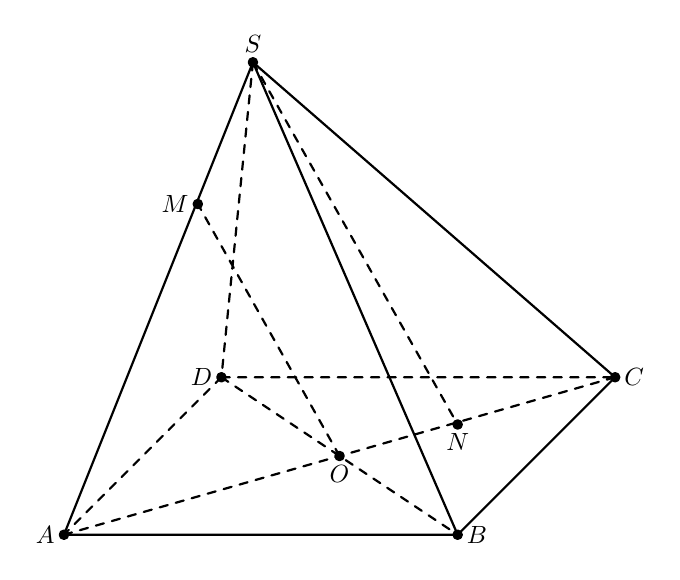
\begin{tikzpicture}[line join=round, line cap=round,>=stealth,thick]
				\coordinate (A) at (-4,-2);
				\coordinate (B) at (1,-2);
				\coordinate (C) at (3,0);
				\coordinate (D) at (-2,0);
				\coordinate (S) at (-1.6,4);
				\coordinate (N) at (1,-0.6);
				\coordinate (M) at (-2.3,2.2);
				\coordinate (O) at (intersection of D--B and A--C);
				\draw[dashed](S)--(D) (D)--(A) (D)--(C) (D)--(B) (A)--(C) (S)--(N) (O)--(M);
				\draw(S)--(A) (A)--(B) (S)--(B) (S)--(C) (B)--(C);
				\foreach \i in {S,A,B,C,D,M,N,O}{\draw[fill=](\i) circle (1.5pt);}
				\foreach \i in {S}{\draw(\i) node[scale=0.9,above]{$\i$};}
				\foreach \i in {M,D,A}{\draw(\i) node[scale=0.9, left]{$\i$};}
				\foreach \i in {O,N}{\draw(\i) node[scale=0.9,below]{$\i$};}
				\foreach \i in {B,C}{\draw(\i) node[scale=0.9, right]{$\i$};}
			\end{tikzpicture}
		\end{center}
		\begin{itemchoice}
			\itemch \textbf{Đúng}. Trong mặt phẳng $(SAC)$ kẻ $SN$ song song $OM$ với $N$ thuộc $AC$. Khi đó $N$ thuộc mặt phẳng $(ABCD)$ nên $N$ là hình chiếu song song của $S$ lên mặt phẳng $(ABCD)$ theo phương $OM$.
			\itemch \textbf{sai}. Tam giác $SAN$ có $OM \parallel SN \Rightarrow \dfrac{AM}{AS}=\dfrac{AO}{AN}=\dfrac{2}{3}.\quad(1)$.
			\itemch \textbf{sai}. Suy ra $\dfrac{\dfrac{1}{2}AC}{AN}=\dfrac{2}{3} \Rightarrow \dfrac{AC}{AN}=\dfrac{4}{3} \Rightarrow \dfrac{AN}{AC}=\dfrac{3}{4}.\quad(2)$.
			\itemch \textbf{Đúng}. Từ $(1)$, $(2)$ suy ra $\dfrac{CN}{CA}=\dfrac{1}{4}$.
		\end{itemchoice}
	}
\end{ex}
%%==========Câu 4
\begin{ex}%[1H4H6-3]
Cho hình lập phương $ABCD.A'B'C'D'$. Gọi $M, N, P$ lần lượt là trung điểm $AD, BC$ và $CC'$.
\choiceTF
{\True $BD$ song song $B'D'$ và $DA'$ song song $CB'$}
{\True$(A'BD)$ song song $(B'CD')$}
{\True$(MNP)$ song song $(ABC')$}
{Thiết diện của hình lập phương khi cắt bởi mặt phẳng $(MNP)$ là hình thang cân}
\loigiai{
	\begin{center}
		\begin{tikzpicture}[scale=1, font=\footnotesize, line join=round, line cap=round, >=stealth]
		\def\bc{4} % cạnh BC
		\def\ba{2} % cạnh BA
		\def\h{4} % đường cao
		\def\gocB{35} % góc B của đáy
		\coordinate[label=below left:$B$] (B) at (0,0);
		\coordinate[label=above left:$A$] (A) at (\gocB:\ba);
		\coordinate[label=below:$C$] (C) at (\bc,0);
		\coordinate[label=right:$D$] (D) at ($(C)-(B)+(A)$);
		\coordinate[label=above left:$A'$] (A') at ($(A)+(90:\h)$);
		\coordinate[label=left:$B'$] (B') at ($(B)-(A)+(A')$);
		\coordinate[label=below right:$C'$] (C') at ($(C)-(A)+(A')$);
		\coordinate[label=right:$D'$] (D') at ($(D)-(A)+(A')$);
		\coordinate[label=below:$M$] (M) at ($(D)!.5!(A)$);
		\coordinate[label=below:$N$] (N) at ($(B)!.5!(C)$);
		\coordinate[label=left:$P$] (P) at ($(C)!.5!(C')$);
		\coordinate[label=right:$Q$] (Q) at ($(D)!.5!(D')$);
		\draw (B')--(B)--(C)--(D)--(D')--(A')--(B')--(C')--(D') (C)--(C')(N)--(P)--(Q);
		\draw[dashed] (A')--(A)--(D) (A)--(B)(Q)--(M)--(N);
		\foreach \diem in {A,B,C,D,A',B',C',D',M,N,P,Q}	\fill (\diem)circle(1.5pt);
		\end{tikzpicture}
		\end{center}
	\begin{itemchoice}
		\itemch Đúng. Vì $BDD'B'$ là hình bình hành nên $BD\parallel B'D'$.
		Tương tự, ta có $DA'\parallel CB'$.
		\itemch Đúng. Vì $BD\parallel B'D'$ và $DA'\parallel CB'$.
		Suy ra $(A'BD)\parallel (B'CD')$.\\
		\itemch Đúng. Ta có $AB\parallel MN$ và $BC'\parallel NP$	nên $(ABC')\parallel (MNP)$.
		\itemch Sai. Ta có $MN\subset (MNP)$, $CD\subset( DCC'D')$, $P\in (MNP)\cap (DCC'D')$ và $MN \parallel DC$ nên giao tuyến của $(MNP)$ và $(DCC'D')$ là đường thẳng qua $P$ và song song $CD$.\\
		Gọi $Q$ là trung điểm $DD'$ thì $PQ$ là giao tuyến của $(MNP)$ và $(DCC'D')$.\\
		Vậy thiết diện là $MNPQ$.\\
		Vì $MN\parallel PQ, MN=PQ$ nên thiết diện là hình hình hành.
	\end{itemchoice}
}
\end{ex}

\Closesolutionfile{ans}
\indapan{3}{ans/ans-1-C4-B5-DE1-DS}

\Opensolutionfile{ans}[ans/ans-1-C4-B5-DE1-KQ]
\caukq
%%==========Câu 1
\begin{ex}%[1H4H6-3]
Cho tứ diện $ABC D$. Điểm $G$ là trọng tâm của tam giác $ABC$ và $M$ là trung điểm $A B$. Hình chiếu song song của điểm $M$ và $G$ theo phương $C D$ lên mặt phẳng $(ABD)$ là $E$. Khi đó $\overrightarrow{MA}+\overrightarrow{MB}+\overrightarrow{MD}=k\overrightarrow{ME}$. Với điểm $M$ bất kỳ, giá trị của $k$ bằng
\shortans{$3$}
	\loigiai{
		Vì $M$ thuộc mặt phẳng $(ABD)$ nên hình chiếu song song của $M$ theo phương $C D$ lên mặt phẳng $(ABD)$ cũng là chính nó.\\
		Gọi $E$ là trọng tâm tam giác $ABD$. Vì $G$, $E$ lần lượt là trọng tâm của tam giác $ABC$, $ABD$ nên $\dfrac{MG}{MC}=\dfrac{ME}{MD}=\dfrac{1}{3} \Rightarrow GE \parallel CD$ (định lí Thalès).\\
		Vậy hình chiếu song song của điểm $G$ theo phương $CD$ lên mặt phẳng $(ABD)$ là trọng tâm $E$ của tam giác $ABD$.\\
	Khi đó với điểm $M$ bất kỳ, ta có $\overrightarrow{MA}+\overrightarrow{MB}+\overrightarrow{MD}=3\overrightarrow{ME}$ nên giá trị của $k$ bằng $3$.}
\end{ex}

%%==========Câu 2
\begin{ex}%[1H4V6-3]
	Cho hình chóp $S.ABCD$, đáy là hình thang ($AB\parallel CD$). Gọi $M$ là trung điểm của $SB$. Mặt phẳng qua $DM$, song song với $AB$ cắt đường thẳng $SC$ tại $Q$. Tính tỉ số $\dfrac{SC}{SQ}$.
\shortans{$1$}
	\loigiai{
		\immini{
			Gọi $(\alpha)$ là mặt phẳng qua $DM$ và song song với $AB$. \\
			Vì $AB\parallel(\alpha)$ và $AB\subset(ABCD)$ nên giao tuyến của $(\alpha)$ và $(ABCD)$ là đường thẳng qua $D$ và song song với $AB$. Ta có $DC\parallel AB$ nên $DC$ chính là giao tuyến của $(\alpha)$ và $(ABCD)$. Do đó $(\alpha)$ cắt $SC$ tại $C$, tức là $Q$ trùng với $C$. Vì vậy $\dfrac{SC}{SQ}=1$. }{
			\begin{tikzpicture}[scale=1, font=\footnotesize, line join=round, line cap=round, >=stealth]
			\def\bc{4} % cạnh BC
			\def\ba{2} % cạnh BA
			\def\h{4} % đường cao
			\def\gocB{30} % góc B của đáy
			\coordinate[label=below left:$B$] (B) at (0,0);
			\coordinate[label=above left:$A$] (A) at (\gocB:\ba);
			\coordinate[label=below:$C$] (C) at (\bc,0);
			\coordinate[label=right:$D$] (D) at ($.8*(A)-.8*(B)+(C)$);
			\coordinate[label=above:$S$] (S) at ($(A)+(0:.5)+(90:\h)$);
			\coordinate[label=left:$N$] (N) at ($(A)!.5!(S)$);
			\coordinate[label=left:$M$] (M) at ($(B)!.5!(S)$);
			\draw (B)--(C)--(D)--(S)--cycle (S)--(C)--(M);
			\draw[dashed] (A)--(D)--(M)--(N)--(D) (S)--(A)--(B);
			\foreach \diem in {A,B,C,D,S,M,N}	\fill (\diem)circle(1.5pt);
			\end{tikzpicture}
		}
	}
\end{ex}

%%==========Câu 3
\begin{ex}%[1H4V6-3]
Cho lăng trụ tam giác $ABC.A' B' C$. Trên đường thẳng $B A$ lấy điểm $M$ sao cho $A$ nằm giữa $B$ và $M$, $M A=\dfrac{1}{2} $A$ B$. Gọi $E$ là trung điểm của $A C$. Gọi $D=BC\cap(M B' E)$. Tính tỉ số $\dfrac{B D}{C D}$.
\shortans{$3$}
	\loigiai{
		Trong $(ABB'A')$ gọi $K=M B'\cap AA'$. Trong $(ABC)$ gọi $D=ME\cap CB$.\\ Thiết diện là tứ giác $DEK B'$.
		\begin{center}
	\begin{tikzpicture}[scale=1, font=\footnotesize, line join=round, line cap=round, >=stealth]
	\def\ac{4} % cạnh AC
	\def\ab{2} % cạnh AB
	\def\ben{4} % cạnh bên
	\def\gocnghieng{75} % góc nghiêng cạnh bên
	\def\gocA{50} % góc A của đáy
	\coordinate[label=left:$A$] (A) at (0,0);
	\coordinate[label=right:$C$] (C) at (\ac,0);
	\coordinate[label=below left:$B$] (B) at (-\gocA:\ab);
	\coordinate[label=left:$A'$] (A') at ($(A)+(\gocnghieng:\ben)$);
	\coordinate[label=above :$B'$] (B') at ($(B)-(A)+(A')$);
	\coordinate[label=right:$C'$] (C') at ($(C)-(A)+(A')$);
	\coordinate[label=left:$M$] (M) at ($(A)+.5*(A)-.5*(B)$);
	\coordinate[label=above:$E$] (E) at ($(A)!.5!(C)$);
	\coordinate[label=below right:$F$] (F) at ($(B)!.5!(C)$);
	\coordinate[label=below right:$D$] (D) at ($(F)+.5*(F)-.5*(B)$);
	\draw (A')--(A)--(B)--(C)--(C')--(A')--(B')--(C') (B)--(B')--(M)--(A) (B')--(D);
	\draw[dashed] (A)--(C) (M)--(D) (F)--(E);
	\foreach \diem in {A,B,C,A',B',C',E,F,D,M} \fill (\diem)circle(1.5pt);
	\end{tikzpicture}	
	\end{center}
		Kẻ $EF\parallel  AB\,(F \in CB)$. Khi đó $E F$ là đường trung bình của tam giác $ABC$ và $E F=\dfrac{A B}{2}$.\\
		Xét tam giác $DBM$ ta có $\dfrac{F D}{B D}=\dfrac{E F}{B M}=\dfrac{1}{3} \Rightarrow FD=\dfrac{1}{2} FB=\dfrac{1}{2} FC$ suy ra $D$ là trung điểm của $F C$ do đó $\dfrac{B D}{C D}=3$.}
\end{ex}

%%==========Câu 4
\begin{ex}%[1H4V6-3]
Cho tứ diện $ABCD$ và $M$ là điểm bất kì thuộc miền trong của tam giác $BCD$. Gọi $B'$, $C'$, $D'$ lần lượt là hình chiếu song song của $M$ theo các phương $AB$, $AC$, $AD$ lên các mặt $(ACD)$, $(ABD)$, $(ABC)$. Tính $\dfrac{MB'}{AB}+\dfrac{MC'}{AC}+\dfrac{MD'}{AD}$.
\shortans{$1$}
	\loigiai{
\immini{
	Trong tam giác $ABI$ ta có $\dfrac{MB'}{AB}=\dfrac{MI}{BI}$.\\
	Tương tự ta cũng có $\dfrac{MC'}{AC}=\dfrac{MJ}{CJ}$ và $\dfrac{MD'}{AD}=\dfrac{MK}{DK}$.\\
	Dễ thấy rằng $\dfrac{S_{MBD}}{S_{CBD}}=\dfrac{MJ}{CJ}$, $\dfrac{S_{MCD}}{S_{BCD}}=\dfrac{MI}{BI}$, $\dfrac{S_{MBC}}{S_{DBC}}=\dfrac{MK}{DK}$.\\
	Cộng các đẳng thức với nhau vế theo vế ta được $$\dfrac{MB'}{AB}+\dfrac{MC'}{AC}+\dfrac{MD'}{AD}=1.$$
}{
	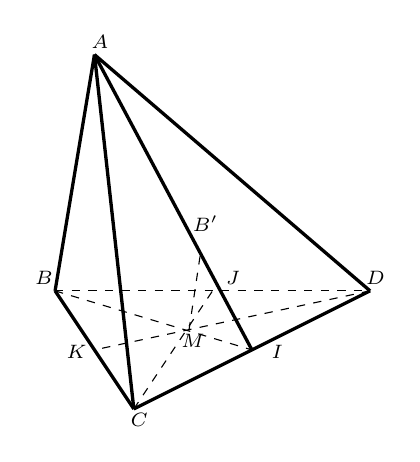
\begin{tikzpicture}[scale=0.5]
	\draw [dashed] (2.,5.)-- (10.,5.);
	\draw [line width=1.2pt] (2.,5.)-- (4.,2.);
	\draw [line width=1.2pt] (4.,2.)-- (10.,5.);
	\draw [line width=1.2pt] (3.,11.)-- (2.,5.);
	\draw [line width=1.2pt] (3.,11.)-- (4.,2.);
	\draw [line width=1.2pt] (3.,11.)-- (10.,5.);
	\draw [line width=1.2pt] (3.,11.)-- (7.,3.5);
	\draw [dashed] (2.,5.)-- (7,3.5);
	\draw [dashed] (10.,5.)-- (3.,3.5);
	\draw [dashed] (4.,2.)-- (6.,5.);
	\draw [dashed] (5.4,4)-- (5.7,6);
	\begin{scriptsize}
	\draw (2.14,5.33) node[left] {$B$};
	\draw (10.14,5.33) node {$D$};
	\draw (4.14,2.1) node [below]{$C$};
	\draw (3.14,11.33) node {$A$};
	\draw (7.3,3.83) node [below right]{$I$};
	\draw (3,3.81) node [below left]{$K$};
	\draw (6.14,5.33) node [right]{$J$};
	\draw (5.5,4.1) node [below]{$M$};
	\draw (5.82,6.31) node [above]{$B'$};
	\end{scriptsize}
	\end{tikzpicture}
}
}
\end{ex}

%%==========Câu 5
\begin{ex}%[1H4V6-3]
Cho tứ diện $ABCD$ và $M$ là điểm bất kì thuộc miền trong của tam giác $BCD$. Gọi $B'$, $C'$, $D'$ lần lượt là hình chiếu song song của $M$ theo các phương $AB$, $AC$, $AD$ lên các mặt $(ACD)$, $(ABD)$, $(ABC)$. Tìm giá trị lớn nhất của $\dfrac{MB'}{AB}\cdot\dfrac{MC'}{AC}\cdot\dfrac{MD'}{AD}$ là $\dfrac{a}{b}$ với $a,b$ nguyên và $(a,b)=1$. Giá trị của $a+b$ bằng
\shortans{$10$}
	\loigiai{
\immini{
	Trong tam giác $ABI$ ta có $\dfrac{MB'}{AB}=\dfrac{MI}{BI}$.\\
	Tương tự ta cũng có $\dfrac{MC'}{AC}=\dfrac{MJ}{CJ}$ và $\dfrac{MD'}{AD}=\dfrac{MK}{DK}$.\\
	Dễ thấy rằng $\dfrac{S_{MBD}}{S_{CBD}}=\dfrac{MJ}{CJ}$, $\dfrac{S_{MCD}}{S_{BCD}}=\dfrac{MI}{BI}$, $\dfrac{S_{MBC}}{S_{DBC}}=\dfrac{MK}{DK}$.\\
	Cộng các đẳng thức với nhau vế theo vế ta được 
	$$\dfrac{MB'}{AB}+\dfrac{MC'}{AC}+\dfrac{MD'}{AD}=1$$
	
}{
	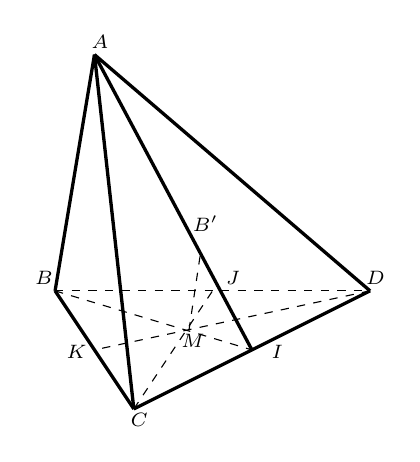
\begin{tikzpicture}[scale=0.5]
	\draw [dashed] (2.,5.)-- (10.,5.);
	\draw [line width=1.2pt] (2.,5.)-- (4.,2.);
	\draw [line width=1.2pt] (4.,2.)-- (10.,5.);
	\draw [line width=1.2pt] (3.,11.)-- (2.,5.);
	\draw [line width=1.2pt] (3.,11.)-- (4.,2.);
	\draw [line width=1.2pt] (3.,11.)-- (10.,5.);
	\draw [line width=1.2pt] (3.,11.)-- (7.,3.5);
	\draw [dashed] (2.,5.)-- (7,3.5);
	\draw [dashed] (10.,5.)-- (3.,3.5);
	\draw [dashed] (4.,2.)-- (6.,5.);
	\draw [dashed] (5.4,4)-- (5.7,6);
	\begin{scriptsize}
	\draw (2.14,5.33) node[left] {$B$};
	\draw (10.14,5.33) node {$D$};
	\draw (4.14,2.1) node [below]{$C$};
	\draw (3.14,11.33) node {$A$};
	\draw (7.3,3.83) node [below right]{$I$};
	\draw (3,3.81) node [below left]{$K$};
	\draw (6.14,5.33) node [right]{$J$};
	\draw (5.5,4.1) node [below]{$M$};
	\draw (5.82,6.31) node [above]{$B'$};
	\end{scriptsize}
	\end{tikzpicture}
}

Theo bất đẳng thức AM-GM cho bộ ba số không âm ta có 
$$\dfrac{MB'}{AB}\cdot\dfrac{MC'}{AC}\cdot\dfrac{MD'}{AD}\leq \left (\dfrac{\dfrac{MB'}{AB}+\dfrac{MC'}{AC}+\dfrac{MD'}{AD}}{3}\right )^3=\dfrac{1}{9}.$$
Dấu bằng xảy ra khi $\dfrac{MB'}{AB}=\dfrac{MC'}{AC}=\dfrac{MD'}{AD}$ hay $\dfrac{MI}{BI}=\dfrac{MJ}{CJ}=\dfrac{MK}{DK}=\dfrac{1}{3}$, tức $M$ là trọng tâm tam giác $ABC$.
}	
\end{ex}

%%==========Câu 6
\begin{ex}%[1H2G4]
	Cho hình chóp $S.ABCD$ đáy là hình bình hành tâm $O$. Điểm $M$ di động trên $SC$ ($M$ không trùng với $S$ và $C$), $(\alpha)$ là mặt phẳng chứa $AM$ và song song với $BD$. Gọi $H$ và $K$ lần lượt là giao điểm của $(\alpha)$ với $SB$ và $SD$. Giá trị của biểu thức $\dfrac{SB}{SH}+\dfrac{SD}{SK}-\dfrac{SC}{SM}$ có giá trị bằng
\shortans{$1$}
	\loigiai{
	\begin{center}
		\begin{tikzpicture}[line cap=round,line join=round,>=triangle 45,x=1.0cm,y=1.0cm]
		\clip(-1.9,0.48) rectangle (4.66,8.06);
		\draw [line width=1.2pt,dash pattern=on 2pt off 2pt] (-1.42,0.82)-- (0.04,3.26);
		\draw [line width=1.2pt,dash pattern=on 2pt off 2pt] (0.04,3.26)-- (4.18,3.3);
		\draw [line width=1.2pt,dash pattern=on 2pt off 2pt] (0.92,7.34)-- (0.04,3.26);
		\draw [line width=1.2pt] (0.92,7.34)-- (-1.42,0.82);
		\draw [line width=1.2pt] (-1.42,0.82)-- (2.72,0.86);
		\draw [line width=1.2pt] (2.72,0.86)-- (4.18,3.3);
		\draw [line width=1.2pt] (0.92,7.34)-- (2.72,0.86);
		\draw [line width=1.2pt] (0.92,7.34)-- (4.18,3.3);
		\draw [line width=1.2pt,dash pattern=on 2pt off 2pt] (-1.42,0.82)-- (4.18,3.3);
		\draw [line width=1.2pt,dash pattern=on 2pt off 2pt] (2.72,0.86)-- (0.04,3.26);
		\draw [line width=1.2pt,dash pattern=on 2pt off 2pt] (0.92,7.34)-- (1.38,2.06);
		\draw [line width=1.2pt,dash pattern=on 2pt off 2pt] (-1.42,0.82)-- (1.38,2.06);
		\draw [line width=1.2pt,dash pattern=on 2pt off 2pt] (1.38,2.06)-- (3.12,4.62);
		\draw [line width=1.2pt,dash pattern=on 2pt off 2pt] (0.46,5.23)-- (1.85,3.99);
		\draw [line width=1.2pt] (1.85,3.99)-- (-1.42,0.82);
		\draw [line width=1.2pt,dash pattern=on 2pt off 2pt] (-1.42,0.82)-- (0.46,5.23);
		\draw [line width=1.2pt,dash pattern=on 2pt off 2pt] (0.46,5.23)-- (2.06,5.93);
		\draw [line width=1.2pt] (2.06,5.93)-- (1.85,3.99);
		\draw (0.7,7.78) node[anchor=north west] {$S$};
		\draw (-1.86,0.92) node[anchor=north west] {$A$};
		\draw (2.78,0.92) node[anchor=north west] {$B$};
		\draw (4.28,3.4) node[anchor=north west] {$C$};
		\draw (-0.34,3.38) node[anchor=north west] {$D$};
		\draw (1.12,1.92) node[anchor=north west] {$O$};
		\draw (2.02,4.18) node[anchor=north west] {$H$};
		\draw (0.62,5.64) node[anchor=north west] {$K$};
		\draw (0.82,4.7) node[anchor=north west] {$I$};
		\draw (2.14,6.16) node[anchor=north west] {$M$};
		\draw (3.22,4.82) node[anchor=north west] {$J$};
		\begin{scriptsize}
		\draw [fill=black] (-1.42,0.82) circle (1.0pt);
		\draw [fill=black] (0.04,3.26) circle (1.0pt);
		\draw [fill=black] (4.18,3.3) circle (1.0pt);
		\draw [fill=black] (2.72,0.86) circle (1.0pt);
		\draw [fill=black] (0.92,7.34) circle (1.0pt);
		\draw [fill=black] (1.38,2.06) circle (1.0pt);
		\draw [fill=black] (2.06,5.93) circle (1.0pt);
		\draw [fill=black] (3.12,4.61) circle (1.0pt);
		\draw [fill=black] (1.16,4.61) circle (1.0pt);
		\draw [fill=black] (0.46,5.23) circle (1.0pt);
		\draw [fill=black] (1.85,3.99) circle (1.0pt);
		\end{scriptsize}
		\end{tikzpicture}
	\end{center}
		Gọi $I$ là giao điểm của $SO$ và $AM$, $J$ là trung điểm của $MC$.\\
		Vì $(\alpha) \parallel BD$ $(\alpha)$ cắt mặt phẳng $(SBD)$ theo giao tuyến là đường thẳng $HK$ đi qua $I$ và song song với $BD$ ($H \in SB$, $K \in SD$).\\
		Theo định lý Ta-lét ta có: $\dfrac{SB}{SH}=\dfrac{SO}{SI}=\dfrac{SD}{SK}$.\\
		Suy ra $\dfrac{SB}{SH}+\dfrac{SD}{SK}-\dfrac{SC}{SM}=\dfrac{2SO}{SI}-\dfrac{SC}{SM}=\dfrac{2SJ}{SM}-\dfrac{SC}{SM}=\dfrac{2SC-2JC-SC}{SM}=\dfrac{SC-2JC}{SM}=\dfrac{SC-MC}{SM}=\dfrac{SM}{SM}=1$.
}
\end{ex}

\Closesolutionfile{ans}
\indapan{6}{ans/ans-1-C4-B5-DE1-KQ}
\subsection{Đề 2}
\Opensolutionfile{ans}[ans/ans-1-C4-B5-DE2]
\caulc
%%==========Câu 1
\begin{ex}%[1H4N6-1]
Qua phép chiếu song song, tính chất nào không được bảo toàn?
\choice
{\True Chéo nhau}
{đồng qui}
{Song song}
{thẳng hàng}
\loigiai{
	Qua phép chiếu song song, tính chất chéo nhau không được bảo toàn}
\end{ex}

%%==========Câu 2
\begin{ex}%[1H4N6-1]
Xét phép chiếu song song lên mặt phẳng $(P)$ theo phương $l$.Trong các mệnh đề  sau mệnh đề nào đúng?
\choice
{Hình chiếu song song của hai đường thẳng cắt nhau có thể song song với nhau}
{\True Hình chiếu song song của hai đường thẳng chéo nhau có thể song song với nhau}
{Hình chiếu song song của hai đường thẳng chéo nhau thì song song với nhau}
{Các mệnh đề trên đều sai}
\loigiai{
	Hình chiếu song song của hai đường thẳng chéo nhau có thể song song với nhau; cũng có thể cắt nhau. Do đó mệnh đề đúng là Hình chiếu song song của hai đường thẳng chéo nhau có thể song song với nhau}
\end{ex}

%%==========Câu 3
\begin{ex}%[1H4N6-1]
Cho tam giác $ABC$ ở trong mp $(\alpha)$ và phương $l$. Biết hình chiếu của tam giác $ABC$ lên mp $(P)$ là một đoạn thẳng. Khẳng định nào sau đây đúng ?
\choice
{$(\alpha)\parallel (P)$}
{$(\alpha)\equiv (P)$}
{\True $(\alpha)\parallel l$ hoặc $(\alpha)\supset l$}
{$A;B;C$ đều sai}
\loigiai{
	Khi phương chiếu $l$ thỏa mãn $(\alpha)\parallel l$ hoặc $(\alpha)\supset l$ thì các đoạn thẳng $AB$, $BC$, $CA$ có hình chiếu lên $(P)$ nằm trên giao tuyến của $(\alpha)$ và $(P)$.}
\end{ex}

%%==========Câu 4
\begin{ex}%[1H4N6-1]
Khẳng định nào sau đây \textbf{sai}?
\choice
{Phép chiếu song song có thể biến đường tròn thành đường tròn}
{Phép chiếu song song có thể biến đường tròn thành đoạn thẳng}
{Phép chiếu song song có thể biến đường tròn thành đường elip}
{\True Phép chiếu song song có thể biến đường tròn thành một điểm}
\loigiai{
	Phương chiếu vuông góc với mặt phẳng chứa đường tròn biến đường tròn thành đường tròn.\\
	Phương chiếu nằm trong mặt phẳng chứa đường tròn biến đường tròn thành đoạn thẳng.\\
	Phương chiếu cắt (không vuông góc) với mặt phẳng chứa đường tròn biến đường tròn thành đường elip}
\end{ex}

%%==========Câu 5
\begin{ex}%[1H4N6-1]
Hãy chọn câu trả lời đúng. Trong không gian
\choice
{Hình biểu diễn của một đoạn thẳng là một đoạn thẳng hoặc một điểm}
{\True Hình biểu diễn của một hình tròn là một hình tròn}
{Hình biểu diễn của một hình chữ nhật là một hình chữ nhật hoặc một đoạn thẳng}
{Hình biểu diễn của một góc là một góc bằng nó}
	\loigiai{
		
	}
\end{ex}

%%==========Câu 6
\begin{ex}%[1H4N6-1]
Hình chiếu của hình chữ nhật không thể là hình nào trong các hình sau?
\choice
{Hình bình hành}
{Hình chữ nhật}
{Hình thoi}
{\True Hình thang}
\loigiai{
	Hình chữ nhật có hai cặp cạnh đối song song nên hình chiếu của nó không thể là hình thang.}
\end{ex}

%%==========Câu 7
\begin{ex}%[1H2B5-1]
	Hình vẽ nào sau đây không phải là hình biểu diễn của hình chóp tứ giác $S.ABCD$?
	\choice
	{\begin{tikzpicture}[scale=1, font=\footnotesize, line join=round, line cap=round, >=stealth]
		\def\ad{4} % cạnh AD
		\def\ab{2} % cạnh AB
		\def\bc{2} % chéo AC
		\def\as{2} % cạnh AS
		\def\gocA{50} % góc A của đáy
		\def\gocB{120} % góc B của đáy
		\coordinate[label=left:$A$] (A) at (0,0);
		\coordinate[label=below left:$B$] (B) at (-\gocA:\ab);
		\coordinate[label=below right:$C$] (C) at ($(B)+(180-\gocA-\gocB:\bc)$);
		\coordinate[label=right:$D$] (D) at (\ad,0);
		\coordinate[label=above:$S$] (S) at (75:\as); % chỉnh 75 và as để thay đổi S
		\draw (A)--(B)--(C)--(D)--(S)--cycle (B)--(S)--(C);
		\draw[dashed] (A)--(D);
		\foreach \diem in {A,B,C,D,S}	\fill (\diem)circle(1.5pt);
		\end{tikzpicture}
	}
	{\begin{tikzpicture}[scale=1, font=\footnotesize, line join=round, line cap=round, >=stealth]
		\def\ad{4} % cạnh AD
		\def\ab{2} % cạnh AB
		\def\bc{2} % chéo AC
		\def\as{2} % cạnh AS
		\def\gocA{50} % góc A của đáy
		\def\gocB{120} % góc B của đáy
		\coordinate[label=left:$A$] (A) at (0,0);
		\coordinate[label=below left:$B$] (B) at (-\gocA:\ab);
		\coordinate[label=below right:$C$] (C) at ($(B)+(180-\gocA-\gocB:\bc)$);
		\coordinate[label=right:$D$] (D) at (\ad,0);
		\coordinate[label=above:$S$] (S) at ($(A)+(-15:2)$); % chỉnh 75 và as để thay đổi S
		\draw (A)--(B)--(C)--(D)--(S)--cycle (B)--(S)--(C) (A)--(D);
		\foreach \diem in {A,B,C,D,S}	\fill (\diem)circle(1.5pt);
		\end{tikzpicture}}
	{\begin{tikzpicture}[scale=1, font=\footnotesize, line join=round, line cap=round, >=stealth]
		\def\ad{4} % cạnh AD
		\def\ab{2} % cạnh AB
		\def\bc{2} % chéo AC
		\def\as{2} % cạnh AS
		\def\gocA{50} % góc A của đáy
		\def\gocB{120} % góc B của đáy
		\coordinate[label=left:$A$] (A) at (0,0);
		\coordinate[label=below left:$B$] (B) at (-\gocA:\ab);
		\coordinate[label=below right:$C$] (C) at ($(B)+(180-\gocA-\gocB:\bc)$);
		\coordinate[label=right:$D$] (D) at (\ad,0);
		\coordinate[label=above:$S$] (S) at ($(A)+(-15:2)$); % chỉnh 75 và as để thay đổi S
		\draw (A)--(B)--(C)--(D)--cycle ;
		\draw[dashed](B)--(S)--(C) (A)--(S)--(D);
		\foreach \diem in {A,B,C,D,S}	\fill (\diem)circle(1.5pt);
		\end{tikzpicture}}
	{\True 
	\begin{tikzpicture}[scale=1, font=\footnotesize, line join=round, line cap=round, >=stealth]
	\def\ad{4} % cạnh AD
	\def\ab{2} % cạnh AB
	\def\bc{2} % chéo AC
	\def\as{2} % cạnh AS
	\def\gocA{50} % góc A của đáy
	\def\gocB{120} % góc B của đáy
	\coordinate[label=left:$A$] (A) at (0,0);
	\coordinate[label=below left:$B$] (B) at (-\gocA:\ab);
	\coordinate[label=right:$D$] (D) at (\ad,0);
	\coordinate[label=above:$S$] (S) at (75:\as); % chỉnh 75 và as để thay đổi S
	\coordinate[label=below right:$C$] (C) at ($(A)!.65!(D)$);
	\draw (A)--(B)--(D)--(S)--cycle (B)--(S);
	\draw[dashed] (A)--(D)(S)--(C)--(B);
	\foreach \diem in {A,B,C,D,S}	\fill (\diem)circle(1.5pt);
	\end{tikzpicture}
}
	\loigiai{
		Hình (D) có 3 điểm $A,B,C$ thẳng hàng $\Rightarrow$ Phương chiếu phải song song với mặt phẳng $(ABC)$, tức là song song với mặt phẳng $(ABCD)$. Khi đó 4 điểm $A,B,C,D$ phải thẳng hàng $\Rightarrow$ (D) sai.}
\end{ex}
%%==========Câu 8
\begin{ex}%[1H2B5-1]
	Hình vẽ nào sau đây \textbf{không phải} là hình biểu diễn của hình hộp?
	\choice
	{\True \begin{tikzpicture}[scale=1, font=\footnotesize, line join=round, line cap=round, >=stealth]
		\def\bc{2} % cạnh BC
		\def\ba{1} % cạnh BA
		\def\h{2.5} % đường cao
		\def\gocB{35} % góc B của đáy
		\coordinate[label=below left:$B$] (B) at (0,0);
		\coordinate[label=above left:$A$] (A) at (\gocB:\ba);
		\coordinate[label=below:$C$] (C) at (\bc,0);
		\coordinate[label=right:$D$] (D) at ($(C)-(B)+(A)$);
		\coordinate (H) at ($(B)!0.4!(D)$); % Hình chiếu của A'
		\coordinate[label=above left:$A'$] (A') at ($(H)+(90:\h)$);
		\coordinate[label=left:$B'$] (B') at ($(B)-(A)+(A')$);
		\coordinate[label=below right:$C'$] (C') at ($(C)-(A)+(A')$);
		\coordinate[label=right:$D'$] (D') at ($(D)-(A)+(A')$);
		\draw (B')--(B)--(C)--(D)--(D')--(A')--(B')--(C')--(D') (C)--(C') (A')--(A)--(B) (A)--(D);
		\foreach \diem in {A,B,C,D,A',B',C',D'}	\fill (\diem)circle(1.5pt);
		\end{tikzpicture}
		}
	{\begin{tikzpicture}[scale=1, font=\footnotesize, line join=round, line cap=round, >=stealth]
		\def\bc{2} % cạnh BC
		\def\ba{1} % cạnh BA
		\def\h{2.5} % đường cao
		\def\gocB{35} % góc B của đáy
		\coordinate[label=below left:$B$] (B) at (0,0);
		\coordinate[label=left:$A$] (A) at (\gocB:\ba);
		\coordinate[label=below:$C$] (C) at (\bc,0);
		\coordinate[label=right:$D$] (D) at ($(C)-(B)+(A)$);
		\coordinate (H) at ($(B)+(95:.4)$); % Hình chiếu của A'
		\coordinate[label=above left:$A'$] (A') at ($(H)+(90:\h)$);
		\coordinate[label=left:$B'$] (B') at ($(B)-(A)+(A')$);
		\coordinate[label= right:$C'$] (C') at ($(C)-(A)+(A')$);
		\coordinate[label=right:$D'$] (D') at ($(D)-(A)+(A')$);
		\draw (B')--(B)--(C)--(D)--(D')--(A')--(B') (A')--(A)--(B) (A)--(D);
		\draw[dashed] (B')--(C')--(D') (C)--(C');
		\foreach \diem in {A,B,C,D,A',B',C',D'}	\fill (\diem)circle(1.5pt);
		\end{tikzpicture}}
	{\begin{tikzpicture}[scale=1, font=\footnotesize, line join=round, line cap=round, >=stealth]
		\def\ba{1} % cạnh BA
		\def\h{2.5} % đường cao
		\coordinate[label=left:$A$] (A) at (0,0);
		\coordinate[label=above:$B$] (B) at ($(A)+(45:\ba)$);
		\coordinate[label=below:$A'$] (A') at ($(A)+(-45:\ba)$);;
		\coordinate[label=below:$D$] (D) at ($(B)-(A)+(A')$);
		\coordinate[label=above:$C$] (C) at ($(B)-(A)+(D)$);
		\coordinate[label=below:$D'$] (D') at ($(A')-(A)+(D)$);
		\coordinate[label=right:$C'$] (C') at ($(C)-(D)+(D')$);
		\draw (A)--(B)--(C)--(D)--(A)--(A')--(D')--(C')--(C) (D)--(D');
		\draw[dashed] (B)--(D)--(A') (C')--(D)--(D');
		\foreach \diem in {A,B,C,D,A',C',D'}	\fill (\diem)circle(1.5pt);
		\end{tikzpicture}
		}
	{\begin{tikzpicture}[scale=1, font=\footnotesize, line join=round, line cap=round, >=stealth]
		\def\ba{4} % cạnh BA
		\def\h{2.5} % đường cao
		\coordinate[label=left:$A$] (A) at (0,0);
		\coordinate[label=right:$C$] (C) at ($(A)+(0:\ba)$);
		\coordinate[label=left:$A'$] (A') at ($(A)+(65:\h)$);;
		\coordinate[label=right:$C'$] (C') at ($(C)-(A)+(A')$);
		\coordinate[label=above:$D$] (D) at ($(A')!.4!(C')$);
		\coordinate[label=above:$B$] (B) at ($(A')!.6!(C')$);
		\coordinate[label=below:$D'$] (D') at ($(A)!.4!(C)$);
		\coordinate[label=below:$B'$] (B') at ($(A)!.6!(C)$);
		\draw (A)--(A')--(C')--(C)--(A)(B')--(B);
		\draw[dashed] (D)--(D');
		\foreach \diem in {A,B,C,D,A',C',D'}	\fill (\diem)circle(1.5pt);
		\end{tikzpicture}
		}
	\loigiai{
		\begin{enumerate}[+]
			\item Rõ ràng (B) đúng.
			\item (C) đúng vì phương chiếu song song với $BD’$.
			\item (D) đúng vì phương chiếu song song với 2 đáy $(ABCD)$ và $(A’B’C’D’)$.
		\end{enumerate}
	}
\end{ex}

%%==========Câu 9
\begin{ex}%[1H2B5-2]
	Cho hình lăng trụ $ABC.A’B’C’$, gọi $I$, $I’$ lần lượt là trung điểm của $AB$, $A’B’$. Qua phép chiếu song song đường thẳng $AI’$, mặt phẳng chiếu $(A’B’C’)$ biến $I$ thành điểm nào sau đây?
	\choice
	{$A’$}
	{\True $B’$}
	{$C’$}
	{$I’$}
	\loigiai{
		\immini{
			Ta có $\heva{&AI\parallel B’I’\\&AI=B’I’}\Rightarrow AIB’I’$ là hình bình hành.\\
			Suy ra qua phép chiếu song song đường thẳng
			$AI’$, mặt phẳng chiếu $(A’B’C’)$ biến điểm $I$
			thành điểm $B’$.}
		{\begin{tikzpicture}[scale=1, font=\footnotesize, line join=round, line cap=round, >=stealth]
			\def\ac{4} % cạnh AC
			\def\ab{2} % cạnh AB
			\def\ben{3} % cạnh bên
			\def\gocnghieng{75} % góc nghiêng cạnh bên
			\def\gocA{50} % góc A của đáy
			\coordinate[label=left:$A$] (A) at (0,0);
			\coordinate[label=right:$C$] (C) at (\ac,0);
			\coordinate[label=below left:$B$] (B) at (-\gocA:\ab);
			\coordinate[label=left:$A'$] (A') at ($(A)+(\gocnghieng:\ben)$);
			\coordinate[label=below right:$B'$] (B') at ($(B)-(A)+(A')$);
			\coordinate[label=right:$C'$] (C') at ($(C)-(A)+(A')$);
			\coordinate[label=below left:$I$] (I) at ($(A)!.5!(B)$);
			\coordinate[label=right:$I'$] (I') at ($(A')!.5!(B')$);
			\draw (A')--(A)--(B)--(C)--(C')--(A')--(B')--(C') (B)--(B')--(I)(A)--(I');
			\draw[dashed] (A)--(C);
			\foreach \diem in {A,B,C,A',B',C',I,I'} \fill (\diem)circle(1.5pt);
			\end{tikzpicture}
	}}
\end{ex}
%%==========Câu 10

\begin{ex}%[1H2B5-3]
	Xét phép chiếu theo phương $d$ lên mặt phẳng $(P)$. $AB\parallel CF$ và $AB=DF$.\\
	Gọi $A’,B’,C’,D’,E’,F’$ lần lượt là hình chiếu của $A,B,C,D,E,F$ qua phép chiếu nói trên. Mệnh đề nào sau đây đúng?
	\choice
	{$\dfrac{DF}{AB}=\dfrac{D’F’}{A’B’}=1$}
	{$\dfrac{C’D’}{C’E’}=\dfrac{CD}{CE}$}
	{$D’F’=A’B’$}
	{\True Tất cả (A), (B), (C) đều đúng}
	\loigiai{
		\immini{
			Vận dụng các tính chất của phép chiếu song song.}
		{\begin{tikzpicture}[scale=.5,line join=round,line width=.7pt,font=\footnotesize,scale=1]
				\path (0,0) coordinate (P) ++(60:4) coordinate (Q)++(0:9) coordinate (M)++(-120:4) coordinate (N)
				($(P)!.4!(N)$) coordinate (P') ($(M)!.4!(N)$) coordinate (Q')
				($(P')!.4!(Q')$) coordinate (A') ($(P')!.7!(Q')$) coordinate (B')
				($(A')+(100:2.5)$) coordinate (A) ($(B')+(100:3)$) coordinate (B)
				($(A')+(160:3)$) coordinate (C') ($1.5*(B')-1.5*(A')+(C')$) coordinate (F')
				($1.3*(A)-1.3*(A')+(C')$) coordinate (C) ($1.3*(B)-1.3*(B')+(F')$) coordinate (F)
				($(C)!1/3!(F)$) coordinate (D) ($(C)!2/3!(F)$) coordinate (E)
				($(C')!1/3!(F')$) coordinate (D') ($(C')!2/3!(F')$) coordinate (E');
				\coordinate (Q') at (intersection of Q--M and C--C');
				\coordinate (M') at (intersection of Q--M and B--B');
				\coordinate (F'') at (intersection of A--B and F--F');
				\coordinate (F''') at (intersection of A--A' and C'--F');
				\draw[shorten <= -5mm,shorten >= -20mm] ($(C')!-2/3!(F')$)--node[pos=1.4,left]{$d$}($(C)!-2/3!(F)$);	
				\draw (M')--(M)--(N)--(P)--(Q)--(Q') (A')--(A)--(B)--(B') (C')--(C)--(F)--(F'') (D)--(D') (E)--(E');
				\draw[dashed] (Q')--(M') (F')--(F'');
				\draw[shorten <= -7mm,shorten >= -5mm] (A')--(B');
				\draw[shorten <= -7mm] (C')--(F''');
				\draw[shorten >= -5mm,dashed] (F''')--(F');
				\draw[cyan] ($(P)!5mm!(Q)$)to [out=0,in=90]($(P)!5.5mm!(N)$);
				\foreach \p/\g in {P/30,A/-150,B/45,C/100,D/100,E/100,F/100,A'/-80,B'/-80,C'/-80,D'/-80,E'/-80,F'/-80}
				\draw[fill=black] (\p) node[shift={(\g:.3)}]{$\p$};
			\end{tikzpicture}
	}}
\end{ex}

%%==========Câu 11
\begin{ex}%[1H2K3-2]
	Cho tứ diện $ABCD$. Gọi $G$, $G'$ lần lượt là trọng tâm $\Delta ABD$ và $\triangle BCD$. Khẳng định nào sau đây là sai?	
	\choice
	{$GG'\parallel(ACD)$}
	{\True $GG'\parallel BD$}
	{$GG'\parallel(ABC)$}
	{$GG'\parallel AC$}
	\loigiai{
		\immini{
			Ta có $GG'$ cắt mặt phẳng $(ABD)$ tại $G$. Do đó $GG'$ không thể song song được với $BD$ nằm trong mặt phẳng $(ABD)$.
		}{\begin{tikzpicture}[scale=1, font=\footnotesize, line join=round, line cap=round, >=stealth]
		\def\ac{4} % cạnh AC
		\def\ab{2} % cạnh AB
		\def\as{3} % cạnh AS
		\def\gocA{50} % góc A của đáy
		\coordinate[label=left:$A$] (A) at (0,0);
		\coordinate[label=right:$C$] (C) at (\ac,0);
		\coordinate[label=below left:$B$] (B) at (-\gocA:\ab);
		\coordinate[label=above:$D$] (D) at (70:\as);
		\coordinate[label=right:$M$] (M) at ($(C)!.5!(D)$);
		\coordinate[label=left:$N$] (N) at ($(A)!.5!(D)$);
		\coordinate[label=right:$G'$] (G') at ($(B)!2/3!(M)$);
		\coordinate[label=left:$G$] (G) at ($(B)!2/3!(N)$);
		\draw (A)--(B)--(C)--(D)--cycle (D)--(B)--(M)(N)--(B);
		\draw[dashed] (A)--(C)(G)--(G')(N)--(M);
		\foreach \diem in {A,B,C,D,M,N,G,G'}\fill (\diem)circle(1.5pt);
		\end{tikzpicture}	
	}}
\end{ex}


%%==========Câu 11
\begin{ex}%[1H2G3]
	Cho hình chóp $S.ABCD$ có đáy $ABCD$ là hình bình hành. Trên các cạnh $BC$, $AD$, $SD$ lần lượt lấy các điểm $M$, $N$, $P$ sao cho $\dfrac{BM}{BC}=\dfrac{AN}{AD}=\dfrac{SP}{SD}$. Gọi $Q$ là giao điểm của đường thẳng $SC$ và mặt phẳng $\left(MNP\right)$. Tứ giác $MNPQ$ là hình gì?
	\choice
	{Hình vuông }
	{Hình bình hành}
	{\True Hình thang}
	{Hình thoi}
	\loigiai{
		\begin{center}
			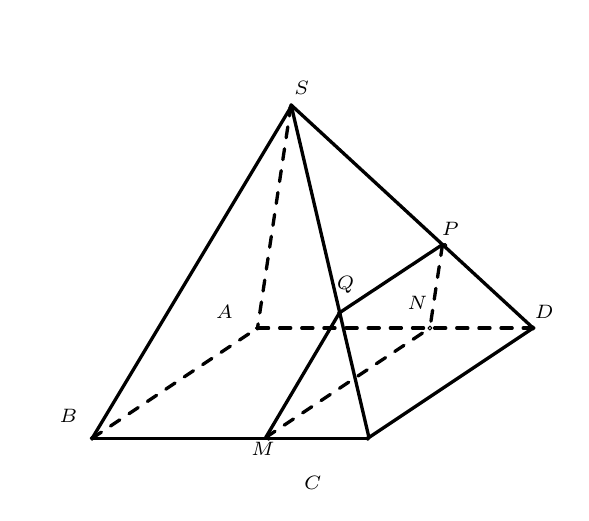
\begin{tikzpicture}[line cap=round,line join=round,>=stealth, scale=0.7,x=1.0cm,y=1.0cm]
			\clip(-0.17,0.014) rectangle (9.5,8.45);
			\draw [line width=1.2pt,dash pattern=on 4pt off 4pt] (4.609,7.048)-- (4.,3.);
			\draw [line width=1.2pt] (4.609,7.048)-- (9.,3.);
			\draw [line width=1.2pt] (4.609,7.048)-- (6.019,1.026);
			\draw [line width=1.2pt] (4.6,7.)-- (1.,1.);
			\draw [line width=1.2pt,dash pattern=on 4pt off 4pt] (1.,1.)-- (4.,3.);
			\draw [line width=1.2pt,dash pattern=on 4pt off 4pt] (4.,3.)-- (9.,3.);
			\draw [line width=1.2pt] (6,1)-- (9.,3.);
			\draw [line width=1.2pt] (6,1)-- (1.,1.);
			\draw [line width=1.2pt,dash pattern=on 4pt off 4pt] (4.15,1.016)-- (7.128,3.);
			\draw [line width=1.2pt] (5.49,3.282)-- (4.15,1.016);
			\draw [line width=1.2pt] (5.491,3.28)-- (7.356,4.515);
			\draw [line width=1.2pt,dash pattern=on 4pt off 4pt] (7.356,4.515)-- (7.128,3.);
			\begin{scriptsize}
			\draw  (4.,3.) circle (1.0pt);
			\draw (3.4,3.3) node {$A$};
			\draw (1.,1.) circle (1.0pt);
			\draw (0.57,1.4) node {$B$};
			\draw  (6.0,1.0) circle (1.0pt);
			\draw (5.,0.2) node {$C$};
			\draw  (9.,3.) circle (1.0pt);
			\draw (9.2,3.3) node {$D$};
			\draw  (4.6,7.0) circle (1.0pt);
			\draw (4.8,7.35) node {$S$};
			\draw  (4.2,1.) circle (1.0pt);
			\draw (4.1,0.8) node {$M$};
			\draw (7.128352260487347,3.) circle (1.0pt);
			\draw (6.9,3.45) node {$N$};
			\draw  (7.4,4.5) circle (1.0pt);
			\draw(7.5,4.8) node {$P$};
			\draw (5.49,3.28) circle (1.0pt);
			\draw(5.6,3.78) node {$Q$};
			\end{scriptsize}
			\end{tikzpicture}
		\end{center}
		Trên mặt phẳng $\left(SCD\right)$, dựng đường thẳng $Px$ song song với đường thẳng $CD$ và cắt $SC$ tại $Q$. Vì $\dfrac{BM}{BC}=\dfrac{AN}{AD}=\dfrac{SP}{SD}$ nên ta có $MN \parallel AB$ và $NP \parallel SA$.
			
			Vì $\heva{&MN \parallel \left(SAB\right)\\&NP \parallel \left(SAB\right)}$ nên hai mặt phẳng $\left(SAB\right)$ và $\left(MNP\right)$ song song với nhau. Mặt khác $PQ \parallel \left(SAB\right)$ nên $Q \in \left(MNP\right)$. Do đó, $Q= SC \cap \left(MNP\right)$.
			
			Tứ giác $MNPQ$ có $PQ \parallel MN \parallel AB$ nên tứ giác $MNPQ$ là hình thang.  }
\end{ex}

\Closesolutionfile{ans}
\indapan{6}{ans/ans-1-C4-B5-DE2}
\cauds
\Opensolutionfile{ans}[ans/ans-1-C4-B5-DE2-DS]
%%==========Câu 1
\begin{ex}%[1H4V6-5]
	Cho hình chóp $S.ABCD$ có đáy $ABCD$ là hình bình hành tâm $O$. Gọi hai điểm $E, F$ lần lượt trên các cạnh $SB, SC$ sao cho $\dfrac{SF}{SC}=\dfrac{1}{2}$ và $\dfrac{SE}{SB}=\dfrac{2}{3}$.
	\choiceTF
	{\True Hai mặt phẳng $(AEF)$ và $(ABCD)$ cắt nhau theo giao tuyến $d$}
	{$BD$ không song song mặt phẳng $(AEF)$}
	{\True Gọi $J$ là giao điểm của $SD$ và $(AEF)$. Tỷ số $\dfrac{SJ}{SD}=\dfrac{2}{3}$}
	{\True Ba đường thẳng $d, JF$ và $CD$ đồng quy}
	\loigiai{
		\begin{center}
			\begin{tikzpicture}[scale=1, font=\footnotesize, line join=round, line cap=round, >=stealth]
			\def\bc{4} % cạnh BC
			\def\ba{2} % cạnh BA
			\def\h{4} % đường cao
			\def\gocB{30} % góc B của đáy
			\coordinate[label=below left:$A$] (A) at (0,0);
			\coordinate[label=above left:$B$] (B) at (\gocB:\ba);
			\coordinate[label=below:$D$] (D) at (\bc,0);
			\coordinate[label=right:$C$] (C) at ($(D)-(A)+(B)$);
			\coordinate[label=above:$S$] (S) at ($(B)+(0:1)+(90:\h)$);
			\coordinate[label=below left:$O$] (O) at ($(D)!.5!(B)$);
			\coordinate[label=above right:$F$] (F) at ($(C)!.5!(S)$);
			\coordinate[label=left:$E$] (E) at ($(S)!2/3!(B)$);
			\coordinate[label=below:$Q$] (Q) at ($(B)-(C)+(B)$);
			\coordinate[label=below:$N$] (N) at ($(D)-(C)+(D)$);
			\path[name path=sd] (S)--(D); % Đặt tên đoạn thẳng AB là ab
			\path[name path=nf] (N)--(F); % Đặt tên đoạn thẳng CD là cd
			\path[name intersections={of= sd and nf,by=J}]; % Lấy giao điểm của ab và cd đặt tên điểm là M
			\path[name path=sa] (S)--(A); % Đặt tên đoạn thẳng AB là ab
			\path[name path=qf] (Q)--(F); % Đặt tên đoạn thẳng CD là cd
			\path[name intersections={of= sa and qf,by=r}];
			\coordinate[label=right:$J$] (J) at (J);
			\coordinate[label=below:$M$] (M) at ($(E)!.5!(J)$);
			\draw (N)--(D)--(C)--(S)--(A) (S)--(D)(F)--(N)--(Q)--(r) (A)--(J);
			\draw[dashed] (B)--(C)--(A)--(D)--(B) (O)--(S)--(B)--(A)(r)--(F)--(A)--(E)--(J);
			\foreach \diem in {A,B,C,D,S,M,E,F,J,N,Q,O}	\fill (\diem)circle(1.5pt);
			\end{tikzpicture}
		\end{center}
		\begin{itemchoice}
			\itemch Đúng. Ta có $A\in (AEF)\cap (ABCD)$. \\
			Trong mp$(SBC)$, gọi $Q$ là giao điểm $EF$ và $BC$.\\ Ta có $Q\in (AEF)\cap (ABCD)$. \\
			Do đó $AQ$ là giao tuyến $d$ của $(AEF)$ và $(ABCD)$.
			\itemch Sai. Tam giác $SQC$ có $QF$ là trung tuyến và $\dfrac{SE}{SB}=\dfrac{2}{3}$ nên $E$ là trọng tâm tam giác. \\
			Do đó $B$ là trung điểm $QC$, suy ra $QBDA$ là hình bình hành, nên $BD\parallel QA\subset (AEF)$. Vậy $BD\parallel (AEF)$.
			\itemch Đúng. Trong mp$(SAC)$, gọi $M=SO\cap AF$.\\
			Trong mp$(SBD)$, gọi $J=SD\cap EM$. Lúc đó $J=SD\cap (AEF)$. \\
			Tam giác $SAC$ có $AF$ và $SO$ là hai đường trung tuyến nên $M$ là trọng tâm tam giác $SAC$. Suy ra $\dfrac{SM}{SO}=\dfrac{2}{3}$.\\
			Mà $\dfrac{SE}{SB}=\dfrac{2}{3}$ nên $ME$ song song $BO$.\\
			Do đó $\dfrac{SJ}{SD}=\dfrac{2}{3}$.
			\itemch Đúng.  Trong mặt phẳng $(SCD)$, vì $\dfrac{SJ}{SD}\neq \dfrac{SF}{SC}$ nên $JF$ và $CD$ cắt nhau.\\
			Gọi $N=JF\cap CD$.\\
			Ta có $(AEF)\cap (ABCD)=AQ, (AEF)\cap (SCD)=JF$ và $(SCD) \cap (ABCD)=CD$ nên $AQ$ đi qua $N$, hay $AQ, JF, CD$ đồng quy tại $N$.
		\end{itemchoice}
	}
\end{ex}

%%==========Câu 2
\begin{ex}%[1H4V6-3]
	Cho hình chóp $ S.ABCD $ có đáy $ ABCD $ là hình thang có đáy lớn là $ AD $. Gọi $ M $, $ N $ lần lượt là các điểm trên các đoạn thẳng $ SA $ và $ SC $ sao cho  $AM = 2MS$; $CN = 2NS$.
	\choiceTF
	{Đường thẳng $CD$ và mặt phẳng $(SAB)$ không giao nhau}
	{\True Giao tuyến của hai mặt phẳng $(SAD)$ và $(SBC)$ song song với $AD$}
	{\True Đường thẳng $MN$ song song mặt phẳng $(BCD)$}
	{\True Thiết diện của hình chóp $S.ABCD$ cắt bởi mặt phẳng $(BMN)$ là một tứ giác}
	\loigiai{
		\begin{center}
			\begin{tikzpicture}[scale=1, font=\footnotesize, line join=round, line cap=round, >=stealth]
			\def\ac{7} % cạnh AC
			\def\ab{3} % cạnh AB
			\def\as{4.5} % cạnh AS
			\def\gocA{50} % góc A của đáy
			\coordinate[label=left:$A$] (A) at (0,0);
			\coordinate[label=right:$D$] (D) at (\ac,0);
			\coordinate[label=below left:$I$] (I) at (-\gocA:\ab);
			\coordinate[label=above:$S$] (S) at (60:\as);
			\coordinate[label=below left:$B$] (B) at ($(A)!.7!(I)$);
			\coordinate[label=below right:$C$] (C) at ($(D)!.7!(I)$);
			\coordinate[label=left:$M$] (M) at ($(A)!2/3!(S)$);
			\coordinate[label= right:$N$] (N) at ($(C)!2/3!(S)$);
			\coordinate[label=below left:$B$] (B) at ($(A)!.7!(I)$);
			\path[name path=ac] (A)--(C); % Đặt tên đoạn thẳng AB là ab
			\path[name path=bd] (B)--(D); % Đặt tên đoạn thẳng CD là cd
			\path[name intersections={of= ac and bd,by=O}]; % Lấy giao điểm của ab và cd đặt tên điểm là M
			\coordinate[label=below:$O$] (O) at (O);
			\path[name path=so] (S)--(O); % Đặt tên đoạn thẳng AB là ab
			\path[name path=mn] (M)--(N); % Đặt tên đoạn thẳng CD là cd
			\path[name intersections={of= so and mn,by=J}]; % Lấy giao điểm của ab và cd đặt tên điểm là M
			\coordinate[label=below left:$J$] (J) at (J);
			\path[name path=bj] (B)--($(J)+.35*(J)-.35*(B)$); % Đặt tên đoạn thẳng AB là ab
			\path[name path=sd] (S)--(D); % Đặt tên đoạn thẳng CD là cd
			\path[name intersections={of= bj and sd,by=K}]; % Lấy giao điểm của ab và cd đặt tên điểm là M
			\coordinate[label=above right:$K$] (K) at (K);
			\draw (A)--(I)--(D)--(S)--cycle (M)--(B)--(N)--(K) (B)--(S)--(C)--(B);
			\draw[dashed] (C)--(A)--(D)--(B)(O)--(S)(B)--(K)--(M)--(N);
			\foreach \diem in {A,I,D,S,O,B,C,M,N,J,K}\fill (\diem)circle(1.5pt);
			\end{tikzpicture}
			
		\end{center}
		\begin{itemchoice}
			\itemch Sai. Do $ABCD$ là hình thang có $ AB $ và $ CD $ không song song, gọi $I = AB  \cap CD$.\\
			Khi đó, $I \in AB \Rightarrow I \in (SAB)$ nên I là giao điểm.
			\itemch Đúng. Ta có, $S$ là điểm chung của hai mặt phẳng.\\
			Trong hai mặt phẳng $ (SAD) $ và $ (SBC) $ lần lượt có $ AD \parallel BC $.\\
			Nên giao tuyến cần tìm là đường thẳng $ Sx  \parallel  AD  \parallel  BC $.
			\itemch Sai. Ta có, $MN$ không thuộc mp$(BCD)$.\\
			Mà $\dfrac{SM}{SA} = \dfrac{1}{3};\dfrac{SN}{SC} = \dfrac{1}{3}$ nên $ MN \parallel  AC$.\\
			Vậy $ MN \parallel  (ABCD)$ hay $MN \parallel  (BCD)$.
			\itemch Đúng. Gọi $ O=AC \cap BD $. Khi đó, $ SO\cap MN = J  $.\\
			Trong $ (SBD) $ có $ BJ\cap SD $ tại $K$. \\
			Như vậy, thiết diện cận tìm là tứ giác $ BMKN $.
		\end{itemchoice}
		}
\end{ex}

%%==========Câu 3
\begin{ex}%[1H4V6-3]
	Cho hình chóp $ S.ABCD $ có đáy $ ABCD $ là hình bình hành tâm $O$. Gọi $ M $  là trung điểm $ SB $.
	\choiceTF
	{\True Giao tuyến của đường thẳng $ (MCD) $ và mp$ (SAB) $ là đường thẳng qua $M$ và song song $AB$}
	{Ba giao tuyến của ba mặt phẳng $(MAB)$, $(MCD)$, $(ABCD)$ đồng quy}
	{\True Giao điểm $ H $ của đường thẳng $ MD $ và $ (SAC) $ thuộc cạnh $SO$}
	{\True Gọi $ G $ là trọng tâm tam giác $ ACD $, $ L $ là giao điểm của đường thẳng $ AG $ và $ BC $; $ T $ là giao điểm của $ SC $ và $ (AGM) $. Khi đó ba điểm $ L, M, T $ thẳng hàng}
	\loigiai{
		\begin{center}
			\begin{tikzpicture}[scale=1, font=\footnotesize, line join=round, line cap=round, >=stealth]
			\def\bc{4} % cạnh BC
			\def\ba{2.5} % cạnh BA
			\def\h{5} % đường cao
			\def\gocB{40} % góc B của đáy
			\coordinate[label=below left:$B$] (B) at (0,0);
			\coordinate[label=above left:$A$] (A) at (\gocB:\ba);
			\coordinate[label=below:$C$] (C) at (\bc,0);
			\coordinate[label=right:$D$] (D) at ($(C)-(B)+(A)$);
			\coordinate[label=above:$S$] (S) at ($(A)+(0:.5)+(90:\h)$);
			\coordinate[label=below:$O$] (O) at ($(A)!.5!(C)$);
			\coordinate[label=left:$M$] (M) at ($(S)!.5!(B)$);
			\coordinate[label=above right:$H$] (H) at ($(S)!2/3!(O)$);
			\coordinate[label=above:$G$] (G) at ($(D)!2/3!(O)$);
			\coordinate[label=below left:$T$] (T) at ($(S)!2/3!(C)$);
			\coordinate[label=right:$L$] (L) at ($(C)-(B)+(C)$);
			\coordinate[label=right:$N$] (N) at ($(S)!.5!(A)$);
			\draw (B)--(C)--(D)--(S)--cycle (S)--(C) ($(C)!.5!(D)$)--(L);
			\draw[dashed] (C)--(A)--(D)--(B) (O)--(S)--(A)--(B) (A)--($(C)!.5!(D)$)(D)--(M)--(N);
			\draw[red](L)--(M); 
			\foreach \diem in {A,B,C,D,S,G,M,H,T,L,O,N}	\fill (\diem)circle(1.5pt);
			\end{tikzpicture}	
		\end{center}
		\begin{itemchoice}
			\itemch Đúng. Ta có $ M \in (MCD) $ và $ M \in SB \subset (SAB) $  nên $M$ là điểm chung thứ nhất của hai mặt phẳng $ (MCD) $ và $ (SAB) $. \\
			Mặt khác, $ DC \subset (MDC) $, $ AB \subset (SAB) $ và $ AB \parallel CD $. \\
			Nên giao tuyến cần tìm là đường thẳng $ d $ đi qua $ M $ và song song với $ AB $ và cắt $ SA $ tại trung điểm $ N $.
			\itemch Sai. Ta có $(MAB)\cap(MCD)=d$, $(MAB)\cap(ABCD)=AB$,\\$(MCD)\cap(ABCD)=CD$ nên $d\parallel AB\parallel CD$.
			\itemch Đúng. Trong mp$ (SBD) $ gọi $H$ là giao điểm của $ SO $ và $ DM $. \\
			Khi đó $ H \in SO \subset (SAC)$, $H \in DM $ nên $ H = DM \cap (SAC) $.\\
			Suy ra Giao điểm $ H $ của đường thẳng $ MD $ và $ (SAC) $ thuộc cạnh $SO$
			\itemch Đúng. Ta có $ L = AG \cap BC \Rightarrow L \in (AGM) \cap (SBC)$. \\
			Ta có $ M \in SB \subset (SBC) \Rightarrow M \in (AGM) \cap (SBC)$. \\
			Ta có $ N = SG \cap (AGM) \Rightarrow N \in (AGM) \cap (SBC)$. \\
			Từ đó $ L, M, N $ cùng thuộc giao tuyến của hai mặt phẳng $ (AGM) $ và $ (SBC) $ nên $ L, M, N $ thẳng hàng.
		\end{itemchoice}
		}
\end{ex}

%%==========Câu 4
\begin{ex}%[1H4V6-3]
	Cho hình chóp $S.ABCD$ có đáy là hình bình hành, các điểm $M, N, E$ lần lượt là trung điểm của các cạnh $SB, SD$ và $CD$.
	\choiceTF
	{Giao tuyến của mặt phẳng $(SAB)$ và mặt phẳng $(SCD)$ là đường thẳng qua $S$ và song song $BC$}
	{\True $ME \parallel (SAD)$}
	{Hai mặt phẳng $(MBD)$ và $(MAC)$ cắt nhau theo giao tuyến $ME$}
	{Thiết diện của hình chóp $S.ABCD$ khi cắt bởi mặt phẳng $(MNE)$ là một tứ giác lồi}
	\loigiai{
		\begin{itemchoice}
			\itemch Sai. Vì $AB \parallel CD$ nên giao tuyến của $(SAB)$ và $(SCD)$ là $Sx \parallel AB \parallel CD$.
			\itemch Đúng. \begin{center}
				\begin{tikzpicture}[scale=1, font=\footnotesize, line join=round, line cap=round, >=stealth]
				\def\bc{4} % cạnh BC
				\def\ba{2} % cạnh BA
				\def\h{4} % đường cao
				\def\gocB{30} % góc B của đáy
				\coordinate[label=below left:$B$] (B) at (0,0);
				\coordinate[label=above left:$A$] (A) at (\gocB:\ba);
				\coordinate[label=below:$C$] (C) at (\bc,0);
				\coordinate[label=right:$D$] (D) at ($(C)-(B)+(A)$);
				\coordinate[label=above:$S$] (S) at ($(A)+(0:1)+(90:\h)$);
				\coordinate[label=above:$x$] (x) at ($(B)-(A)+(S)$);
				\coordinate[label=left:$F$] (F) at ($(B)!.5!(A)$);
				\coordinate[label=below right:$E$] (E) at ($(C)!.5!(D)$);
				\coordinate[label=left:$M$] (M) at ($(B)!.5!(S)$);
				\draw (B)--(C)--(D)--(S)--cycle (S)--(C) (x)--(S)--($(A)-(B)+(S)$);
				\draw[dashed] (A)--(D) (S)--(A)--(B)(M)--(E)--(F)--(M);
				\foreach \diem in {A,B,C,D,S,M,E,F}	\fill (\diem)circle(1.5pt);
				\end{tikzpicture}
				\end{center}
				Từ $E$ kẻ $EF \parallel AD$. Ta có $(MFE) \parallel (SAD)$ suy ra $ME \parallel (SAD)$.
			\itemch Sai. Gọi $O$ là tâm hình bình hành $ABCD$ suy ra $\heva{&O\in AC\subset(MAC)\\&O\in BD\subset(MBD)}\Rightarrow MO=(MAC)\cap(MBD)$.
			\itemch Sai. Dựng thiết diện của hình chóp $S.ABCD$ khi cắt bởi mặt phẳng $(MNE)$.			\\
			$(MNE) \cap (SCD)=EN$.    \\
			Kẻ $MI \parallel SC$ suy ra $M, N, E, I$ đồng phẳng. Ta có
			$(MNE) \cap (SBC)=SI$.\\
			Trong mặt phẳng $(ABCD)$ có $EI \cap AD=L$.\\
			Trong mặt phẳng $(SAD)$, có $LN \cap SA=P$.\\
			Suy ra $(MNE) \cap (SAD)=NP$, 
			$(MNE) \cap (SAD)=MP$. \\
			Vậy thiết diện cần tìm là ngũ giác $MIENP$.
		\end{itemchoice}
	}
\end{ex}

\Closesolutionfile{ans}
\indapan{3}{ans/ans-1-C4-B5-DE2-DS}

\Opensolutionfile{ans}[ans/ans-1-C4-B5-DE2-KQ]
\caukq
%%==========Câu 1
\begin{ex}%[1H4V6-3]
		Cho tứ diện đều $ABCD$ có cạnh bằng $a$. Gọi $M,N$ lần lượt là trọng tâm của $\Delta ABC$ và $\Delta ABD$. Diện tích thiết diện của tứ diện khi cắt bởi mặt phẳng $(BMN)$ là $\dfrac{a^2\sqrt{a}}{b}$. Khi đó $a+b$ bằng
	\shortans{$27$}
	\loigiai{
	\begin{center}
		\begin{tikzpicture}[scale=1.3]
		\coordinate (A) at (2,3); \coordinate (B) at (0,0);
		\coordinate (C) at (1.5,-2); \coordinate (D) at (4,0);
		\coordinate (E) at ($(A)!.5!(C)$);
		\coordinate (F) at ($(A)!.5!(D)$);
		\draw (A) node[above]{$A$}--(B) node[left]{$B$}--(C) node[below]{$C$}--(D) node[right]{$D$}--cycle;
		\draw (A)--(C);
		\draw (B)-- (E) node[below right]{$E$} -- (F) node[right]{$F$};
		\draw [dashed] (B)--(F); \draw [dashed] (B)--(D);
		\coordinate (M) at ($(B)!2/3!(E)$);
		\coordinate (N) at ($(B)!2/3!(F)$);
		\draw[fill] (M) circle (1.5pt) node[below]{$M$}; 
		\draw[fill] (N) circle (1.5pt) node[above]{$N$};
		\end{tikzpicture}
	\end{center}
	Trong $(ABD)$, $BN$ cắt $AD$ tại $F$. Trong $(ABC), BM$ cắt $AC$ tại $E$.\\
			Do $M,N$ lần lượt là trọng tâm của $\Delta ABD$ nên $E,F$ lần lượt là trung điểm của $AC,AD$.\\
			Tứ diện $ABCD$ có cạnh bằng $a$ nên $BE=BF=\dfrac{a\sqrt{3}}{2}$.\\
			Thiết diện là tam giác cân $BEF$ tại $B$, có cạnh đáy $EF=\dfrac{a}{2}$.\\
			Diện tích $\Delta BEF$ là $S_{BEF}=\dfrac{1}{2}.\dfrac{a}{2}.\sqrt{\left(\dfrac{a\sqrt{3}}{2}\right)^2-\left(\dfrac{a}{4}\right)^2}=\dfrac{a^2\sqrt{11}}{16}$ (đvdt).\\
			Suy ra $a+b=27$.
		}
\end{ex}

%%==========Câu 2
\begin{ex}%[1H4V6-5]
	Cho tứ diện $ABCD$, $M$ là điểm thuộc $BC$ sao cho $MC=2MB$. $N,P$ lần lượt là trung điểm của $BD$ và $AD$. Điểm $Q$ là giao điểm $AC$ với $(MNP)$. Tính $\dfrac{QA}{QC}$.
	\shortans{$0{,}5$}
	\loigiai{
		\begin{center}
			\begin{tikzpicture}[scale=1.25]
			\coordinate (A) at (1.5,3);\coordinate (B) at (0,0);
			\coordinate (C) at (2,-2); \coordinate (D) at (4,-0.5);
			\coordinate (N) at ($(B)!.5!(D)$); \coordinate (P) at ($(A)!.5!(D)$);
			\coordinate (Q) at ($(A)!1/3!(C)$); \coordinate (M) at ($(B)!1/3!(C)$); \coordinate (J) at ($(C)!2!(D)$);
			\draw (A) node[above]{$A$}--(B) node[left]{$B$}--(C) node[below]{$C$}--(D) node[below right]{$D$}--cycle;
			\draw (M) node[below left]{$M$}--(Q) node[left]{$Q$}--(J) node[right]{$J$}--(D); \draw (A)--(C);
			\draw (C)--(P) node[above right]{$P$};
			\draw[dashed] (B)--(D);\draw[dashed] (M)--(J);
			\draw[dashed] (B)--(P);\draw[dashed] (P)--(N) node[below]{$N$};
			\foreach \diem in {A,B,C,D,M,N,P,Q,J}\fill (\diem)circle(1.25pt);
			\end{tikzpicture}
			\end{center}
		$NP$ là đường trung bình của $\Delta ACD \Rightarrow NP \parallel AB$, mà $AB \subset (ABC)\Rightarrow NP \parallel  (ABC)$.\\$P \in(MNP)\cap(ACD).\quad (1)$\\
			Trong $(BCD)$ gọi $J=MN \cap CD$, có $\heva{&J\in MN \subset (MNP)\\ &J\in CD \subset (ACD)}\Rightarrow J\in (MNP) \cap (ACD).\, (2)$\\
			Từ $(1)$ và $(2)$ $\Rightarrow (MNP)\cap(ACD)=JP$. Trong $(ACD)$ gọi $Q=JP\cap AC$, có $\heva{& Q\in AC\\ & Q\in JP \subset (MNP)}\Rightarrow Q=AC\cap (MNP)$.\\
			Có $\heva{& MQ=(MNP)\cap(ABC)\\ & NP\parallel AB; NP \subset (MNP), AB\subset (ABC)} \Rightarrow MQ\parallel NP\parallel AB$.\\
			Theo định lí Ta-lét có $\dfrac{CQ}{CA}=\dfrac{CM}{CB}=\dfrac{2}{3}\Rightarrow \dfrac{QA}{QC}=\dfrac{1}{2}$.
	}
\end{ex}

%%==========Câu 3
\begin{ex}%[1H2G2]
	Hai hình bình hành $ABCD$ và $ABEF$ không cùng nằm trong một mặt phẳng. Trên cạnh $AC$ lấy điểm $M$ và trên cạnh $BF$ lấy điểm $N$ sao cho $\dfrac{AM}{AC}=\dfrac{BN}{BF}=k$. Giá trị $k=\dfrac{a}{b}$ với $a,b\in\mathbb{Z}$ và $(a,b)=1$ để $MN\parallel DE$.
	Tính $a+b$
	\shortans{$4$}
	\loigiai{
	\immini{
			$MN\parallel DE \Rightarrow MN, DE$ đồng phẳng $ \Rightarrow DM, NE$ cắt nhau tại điểm $I$ và $\dfrac{IM}{DM}=\dfrac{IN}{NE}$.\\
			Lại có $\dfrac{IM}{DM}=\dfrac{AI}{DC}=\dfrac{AM}{MC}=\dfrac{k}{1-k};\ \dfrac{IN}{NE}=\dfrac{BI}{EF}=\dfrac{BN}{NF}=\dfrac{k}{1-k}$.\\
			Mặt khác $\dfrac{AI}{DC}+\dfrac{BI}{EF}=\dfrac{AI}{EF}+\dfrac{BI}{EF}=1 \Rightarrow 2.\dfrac{k}{1-k}=1 \Rightarrow k=\dfrac{1}{3}$.\\
			Suy ra $a+b=4$.
		}{
			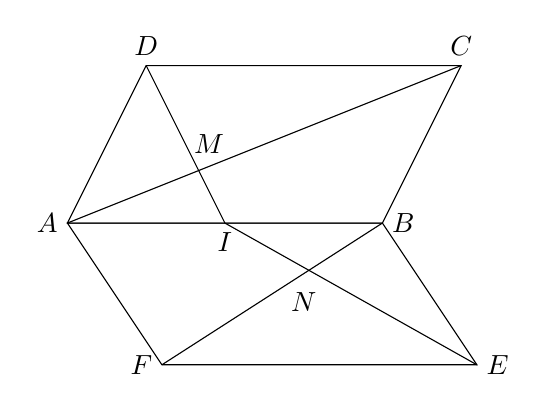
\begin{tikzpicture}[scale=1]
			\coordinate (A) at (0,0);\coordinate (B) at (4,0);
			\coordinate (C) at (5,2);\coordinate (D) at (1,2);
			\coordinate (E) at (5.2,-1.8);\coordinate (F) at (1.2,-1.8);
			\coordinate (I) at (2,0);
			\draw (A) node[left]{$A$}--(B) node[right]{$B$}--(C) node[above]{$C$}--(D) node [above]{$D$}--cycle; 
			\draw (A)--(F) node [left]{$F$}--(E) node[right]{$E$}--(B)--cycle; 
			\draw (A)--(C);\draw (B)--(F); \draw (E)--(I) node [below]{$I$}--(D);
			\draw (1.8,1) node{$M$};\draw (3,-1) node{$N$};
			\end{tikzpicture}}	
	}
\end{ex}

%%==========Câu 4
\begin{ex}%[1H2G5]
	Cho hình hộp $ABCD.A'B'C'D'$. Các điểm $M$, $N$ lần lượt nằm trên các cạnh $B'D$ và $AC$ sao cho $MN \parallel BC'$. Tính tỉ số $\dfrac{MB'}{MD}$.	
	\shortans{$2$}
	\loigiai{
	\immini{ \textbf{\textbullet \quad Xác định vị trí các điểm $M$, $N$.}\\
			Xét phép chiếu song song lên mp $\left(ABCD\right)$ theo phương là đường thẳng $BC'$. Gọi $E$ là ảnh của điểm $B'$ trên mp$\left(ABCD\right)$ qua phép chiếu song song theo phương $BC'$ và $N$ là giao điểm của $DE$ và $AC$. Trên mp $\left(EB'D\right)$, dựng $NM \parallel EB'$ với $M \in B'D$.\\
			\textbullet \quad \textbf{Tính tỉ số $\dfrac{MB'}{MD}$.\\}
			Khi đó, ta có $\dfrac{MB'}{MD}=\dfrac{NE}{ND}=2$ .}
		{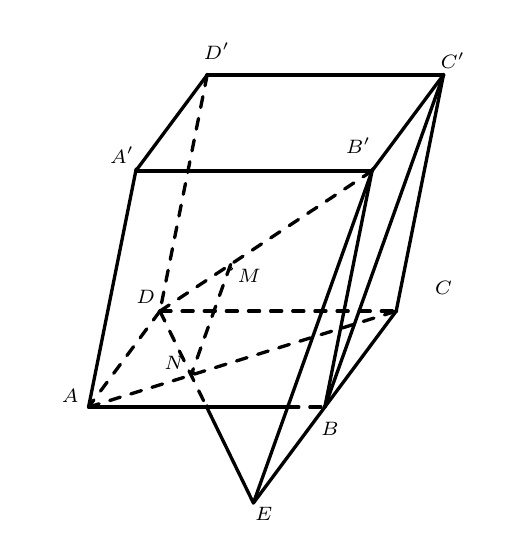
\begin{tikzpicture}[line cap=round,line join=round,>=stealth, scale=0.6,x=1.0cm,y=1.0cm]
			\clip(2.2,3.5) rectangle (12.,14.);
			\draw [line width=1.2pt,dash pattern=on 4pt off 4pt] (5.,8.)-- (10.,8.);
			\draw [line width=1.2pt,dash pattern=on 4pt off 4pt] (5.,8.)-- (3.489,5.969);
			\draw [line width=1.2pt] (8.489,5.969)-- (10.,8.);
			\draw [line width=1.2pt,dash pattern=on 4pt off 4pt] (3.489,5.969)-- (10.,8.);
			\draw [line width=1.2pt,dash pattern=on 4pt off 4pt] (6.,13.)-- (5.,8.);
			\draw [line width=1.2pt] (11.,13.)-- (9.489,10.969);
			\draw [line width=1.2pt] (9.489,10.969)-- (4.489,10.969);
			\draw [line width=1.2pt] (4.489,10.969)-- (3.489,5.969);
			\draw [line width=1.2pt] (4.489,10.969)-- (6.,13.);
			\draw [line width=1.2pt] (6.,13.)-- (11.,13.);
			\draw [line width=1.2pt] (11.,13.)-- (10.,8.);
			\draw [line width=1.2pt] (9.489,10.969)-- (8.489,5.969);
			\draw [line width=1.2pt] (11.,13.)-- (8.489,5.969);
			\draw [line width=1.2pt] (6.978,3.939)-- (8.489,5.969);
			\draw [line width=1.2pt,dash pattern=on 4pt off 4pt] (5.,8.)-- (9.489,10.969);
			\draw [line width=1.2pt] (9.489,10.969)-- (6.978,3.939);
			\draw [line width=1.2pt] (3.489,5.969)-- (7.703,5.969);
			\draw [line width=1.2pt,dash pattern=on 4pt off 4pt] (7.705,5.969)-- (8.489,5.969);
			\draw [line width=1.2pt,dash pattern=on 4pt off 4pt] (5.,8.)-- (5.989,5.969);
			\draw [line width=1.2pt] (5.989,5.969)-- (6.978,3.939);
			\draw [line width=1.2pt,dash pattern=on 4pt off 4pt] (6.496,8.989)-- (5.659,6.646);
			\begin{scriptsize}
			\draw (3.5,6) circle (1.0pt);
			\draw (3.1,6.2) node {$A$};
			\draw(5.,8.) circle (1.0pt);
			\draw (4.7,8.3) node {$D$};
			\draw (10.,8.) circle (1.0pt);
			\draw (11,8.5) node {$C$};
			\draw (8.5,6) circle (1.0pt);
			\draw (8.6,5.5) node {$B$};
			\draw (6.,13.) circle (1.0pt);
			\draw (6.2,13.5) node {$D'$};
			\draw(11.,13.) circle (1.0pt);
			\draw (11.2,13.3) node {$C'$};
			\draw  (9.5,11) circle (1.0pt);
			\draw (9.2,11.5) node {$B'$};
			\draw (4.5,11) circle (1.0pt);
			\draw (4.2,11.3) node {$A'$};
			\draw  (7,4) circle (1.0pt);
			\draw (7.2,3.7) node {$E$};
			\draw (5.7,6.7) circle (1.0pt);
			\draw (5.3,6.9) node {$N$};
			\draw (6,6) circle (0.5pt);
			\draw (7.7,6) circle (0.5pt);
			\draw  (6.5,8.9) circle (1.0pt);
			\draw (6.89,8.75) node {$M$};
			\end{scriptsize}
			\end{tikzpicture}}	
	}
\end{ex}

%%==========Câu 5
\begin{ex}%[1H2G1]
	Cho hình chóp $S.ABCD$ có đáy $ABCD$ là hình bình hành tâm $O$. Gọi $M$ là trung điểm của $SB$ và $G$ là trọng tâm của tam giác $SAD$. Giả sử $H$ là giao điểm của đường thẳng $DM$ với $\left(SAC\right)$. Tính tỉ số $HO:HS$.
	\shortans{$0{,}5$}
	\loigiai{
	\immini{			
			Gọi $H=DM\cap SO$, ta suy ra $\heva{& H \in DM\\& H \in SO \subset \left(SAC\right)}$
			
			$ \Rightarrow H \in \left(SAC\right)$.\\ Do đó, $H =DM \cap \left(SAC\right)$.
			
			Tam giác $SBD$ có 2 trung tuyến $SO$ và $DM$ nên $H$ là trọng tâm của tam giác $SBD$, suy ra $\dfrac{HO}{HS}=\dfrac{1}{2}.$}
		{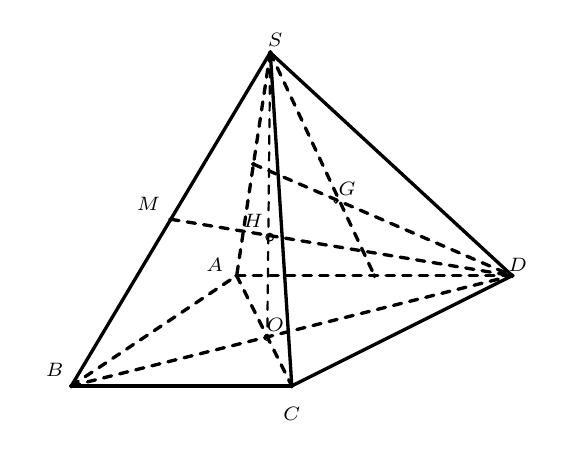
\begin{tikzpicture}[line cap=round,line join=round,>=stealth, scale=0.7,x=1.0cm,y=1.0cm]
			\clip(0.208,0.275) rectangle (9.49,7.5);
			\draw [line width=1.2pt,dash pattern=on 3pt off 3pt] (4.609,7.048)-- (4.,3.);
			\draw [line width=1.2pt] (4.609,7.048)-- (9.,3.);
			\draw [line width=1.2pt] (4.609,7.048)-- (5.,1.);
			\draw [line width=1.2pt] (4.609,7.048)-- (1.,1.);
			\draw [line width=1.2pt,dash pattern=on 3pt off 3pt] (1.,1.)-- (4.,3.);
			\draw [line width=1.2pt,dash pattern=on 3pt off 3pt] (4.,3.)-- (9.,3.);
			\draw [line width=1.2pt] (5.,1.)-- (9.,3.);
			\draw [line width=1.2pt] (5.,1.)-- (1.,1.);
			\draw [line width=1.2pt,dash pattern=on 3pt off 3pt] (1.,1.)-- (9.,3.);
			\draw [line width=1.2pt,dash pattern=on 3pt off 3pt] (4.,3.)-- (5.,1.);
			\draw [line width=1.2pt,dash pattern=on 3pt off 3pt] (4.609,7.048)-- (6.5,3.);
			\draw [line width=1.2pt,dash pattern=on 3pt off 3pt] (4.304,5.024)-- (9.,3.);
			\draw [line width=0.8pt,dash pattern=on 3pt off 3pt] (4.608,7.048)-- (4.555,1.888);
			\draw [line width=1.2pt,dash pattern=on 3pt off 3pt] (2.805,4.024)-- (9.,3.);
			\begin{scriptsize}
			\draw  (4.,3.) circle (1.0pt);
			\draw (3.6,3.2) node {$A$};
			\draw  (1.,1.) circle (1.0pt);
			\draw (0.7,1.3) node {$B$};
			\draw (5.,1.) circle (1.0pt);
			\draw (5,0.5) node {$C$};
			\draw  (9.,3.) circle (1.0pt);
			\draw (9.1,3.2) node {$D$};
			\draw  (4.61,7.05) circle (1.0pt);
			\draw (4.7,7.27) node {$S$};
			\draw  (4.55,1.88) circle (1.5pt);
			\draw (4.7,2.1) node {$O$};
			\draw  (2.805,4.024) circle (1.0pt);
			\draw (2.4,4.3) node {$M$};
			\draw  (4.305,5.024) circle (1.0pt);
			\draw  (6.5,3.) circle (1.0pt);
			\draw  (5.8,4.349) circle (1.0pt);
			\draw(6.0,4.57) node {$G$};
			\draw (4.6,3.7) circle (2.0pt);
			\draw (4.3,4.) node {$H$};
			\end{scriptsize}
			\end{tikzpicture}}	
	}
\end{ex}

%%==========Câu 6
\begin{ex}%[1H2G4]
	Cho hình chóp $S.ABCD$ có đáy là hình thang $AB \parallel CD$, $AB=2CD$. Điểm $M$ thuộc cạnh $AD$ ($M$ không trùng với $A$ và $D$) sao cho $\dfrac{MA}{MD}=x$. Gọi $(\alpha)$ là mặt phẳng qua $M$ và song song với $(SAB)$. Tìm $x$ để diện tích thiết diện của hình chóp cắt bởi mặt phẳng $(\alpha)$ bằng một nửa diện tích tam giác $SAB$	
	\shortans{$1$}
	\loigiai{
	\begin{center}
		\definecolor{ffqqqq}{rgb}{1.,0.,0.}
		\begin{tikzpicture}[scale=.85,line cap=round,line join=round,>=triangle 45,x=1.0cm,y=1.0cm]
		\clip(0.34,-3.42) rectangle (7.74,8.84);
		\fill[line width=0.pt,dash pattern=on 3pt off 3pt,color=ffqqqq,fill=ffqqqq,pattern=north east lines,pattern color=ffqqqq] (2.95,-2.02) -- (3.91,4.69) -- (4.3,5.66) -- (4.56,2.) -- cycle;
		\draw [line width=1.2pt,dash pattern=on 3pt off 3pt] (1.,-3.)-- (3.,2.);
		\draw [line width=1.2pt,dash pattern=on 3pt off 3pt] (3.,2.)-- (7.,2.);
		\draw [line width=1.2pt] (1.,-3.)-- (6.,-0.5);
		\draw [line width=1.2pt] (7.,2.)-- (6.,-0.5);
		\draw [line width=1.2pt,dash pattern=on 3pt off 3pt] (3.,2.)-- (2.57,8.0);
		\draw [line width=1.2pt] (2.57,8.0)-- (1.,-3.);
		\draw [line width=1.2pt] (2.57,8.0)-- (6.,-0.5);
		\draw [line width=1.2pt] (2.57,8.0)-- (7.,2.);
		\draw [line width=1.2pt,dash pattern=on 3pt off 3pt] (4.56,2.)-- (2.95,-2.02);
		\draw [line width=1.2pt] (2.95,-2.02)-- (4.21,6.83);
		\draw [line width=1.2pt] (4.3,5.66)-- (3.91,4.69);
		\draw [line width=1.2pt,dash pattern=on 3pt off 3pt] (4.56,2.)-- (4.3,5.66);
		\draw [line width=1.2pt] (4.3,5.66)-- (4.21,6.83);
		\draw (2.33,8.66) node[anchor=north west] {$S$};
		\draw (2.39,2.23) node[anchor=north west] {$A$};
		\draw (0.46,-2.91) node[anchor=north west] {$B$};
		\draw (6.08,-0.59) node[anchor=north west] {$C$};
		\draw (7.12,2.14) node[anchor=north west] {$D$};
		\draw (4.47,1.76) node[anchor=north west] {$M$};
		\draw (4.35,6.07) node[anchor=north west] {$N$};
		\draw (4.08,7.41) node[anchor=north west] {$E$};
		\draw (3.31,4.55) node[anchor=north west] {$P$};
		\draw (2.86,-2.29) node[anchor=north west] {$Q$};
		\begin{scriptsize}
		\draw [fill=black] (1.,-3.) circle (1.0pt);
		\draw [fill=black] (3.,2.) circle (1.0pt);
		\draw [fill=black] (7.,2.) circle (1.0pt);
		\draw [fill=black] (6.,-0.5) circle (1.0pt);
		\draw [fill=black] (2.57,8.0) circle (1.0pt);
		\draw [fill=black] (4.56,2.) circle (1.0pt);
		\draw [fill=black] (2.95,-2.02) circle (1.0pt);
		\draw [fill=black] (4.3,5.66) circle (1.0pt);
		\draw [fill=black] (3.91,4.69) circle (1.0pt);
		\draw [fill=black] (4.21,6.83) circle (1.0pt);
		\end{scriptsize}
		\end{tikzpicture}
	\end{center}
			Dễ thấy thiết diện là hình thang $MNPQ$ (hình vẽ)\\
			Gọi $E$ là giao điểm của $MN$ và $PQ$.\\
			Ta có: $QM=\dfrac{MD}{AD} \cdot AB+\dfrac{AM}{AD} \cdot CD=\dfrac{1}{x+1}AB+\dfrac{x}{x+1}CD=\dfrac{x+2}{2(x+1)}AB$\\
			Hai tam giác $SAB$ và $EMQ$ đồng dạng nên: $\dfrac{S_{EMQ}}{S_{SAB}}=\left(\dfrac{MQ}{AB} \right)^2=\dfrac{(x+2)^2}{4(x+1)^2}$. (1)\\
			Vì $\dfrac{NP}{CD}=\dfrac{NS}{SD}=\dfrac{AM}{AD}=\dfrac{x}{x+1}$ suy ra $NP=\dfrac{x}{x+1}CD=\dfrac{x}{2(x+1)}AB$.\\
			Do đó $\dfrac{NP}{QM}=\dfrac{x}{x+2}$ và $\dfrac{S_{EPN}}{S_{EMQ}}=\left(\dfrac{NP}{MQ} \right)^2=\dfrac{x^2}{(x+2)^2}$\\
			$\Rightarrow \dfrac{S_{MNPQ}}{S_{EMQ}}=1-\dfrac{x^2}{(x+2)^2} =\dfrac{4x+4}{(x+2)^2}$. (2)\\
			Từ (1) và (2) suy ra $\dfrac{S_{MNPQ}}{S_{ABC}}=\dfrac{4x+4}{4(x+1)^2}=\dfrac{1}{x+1}$.\\
			Vậy $S_{MNPQ}=\dfrac{1}{2}S_{SAB} \Leftrightarrow \dfrac{1}{x+1}=\dfrac{1}{2} \Leftrightarrow x=1$.
	}
\end{ex}

\Closesolutionfile{ans}
\indapan{6}{ans/ans-1-C4-B5-DE2-KQ}
